\documentclass{article}
\usepackage{setspace}
%\usepackage{subfigure}

\pagestyle{plain}
\usepackage{amssymb,graphicx,color}
\usepackage{amsfonts}
\usepackage{latexsym}
\usepackage{a4wide}
\usepackage{amsmath}
\usepackage{paper}
\usepackage{mathtools}
\usepackage{algorithm}
\usepackage{algpseudocode}
\usepackage{cfr-lm}
\usepackage{sectsty}

% \sectionfont{\fontsize{12}{12}\selectfont}
% \subsectionfont{\fontsize{11}{11}\selectfont}
% \subsectionfont{\fontsize{10}{10}\selectfont}
\newtheorem{theorem}{Theorem}
\newtheorem{lemma}[theorem]{Lemma}
\newtheorem{corollary}[theorem]{Corollary}
\newtheorem{proposition}[theorem]{Proposition}
\newtheorem{remark}[theorem]{Remark}
\newtheorem{definition}[theorem]{Definition}
\newtheorem{fact}[theorem]{Fact}

\newtheorem{problem}[theorem]{Problem}
\newtheorem{exercise}[theorem]{Exercise}
\def \set#1{\{#1\} }




\newenvironment{proof}{
PROOF:
\begin{quotation}}{
$\Box$ \end{quotation}}

\usepackage{xcolor}
\newcommand{\jk}[1]{{\color{blue} [JK: #1]}}
\newcommand{\jw}[1]{{\color{gray} [JW: #1]}}
\newcommand{\vw}[1]{{\color{green} [VW: #1]}}

\newcommand{\calF}{\mathcal{F}}
\newcommand{\bbP}{\mathbb{P}}
\newcommand{\bbR}{\mathbb{R}}
\newcommand{\bbD}{\mathbb{D}}
\newcommand{\bbN}{\mathbb{N}}
\newcommand{\bbE}{\mathbb{E}}
\newcommand{\bbV}{\mathbb{V}}
\newcommand{\bbQ}{\mathbb{Q}}
\newcommand{\bbC}{\mathbb{C}}
\newcommand{\calX}{\mathcal{X}}
\newcommand{\calY}{\mathcal{Y}}
\newcommand{\calZ}{\mathcal{Z}}
\newcommand{\calB}{\mathcal{B}}
\newcommand{\calP}{\mathcal{P}}
\newcommand{\calQ}{\mathcal{Q}}
\newcommand{\calS}{\mathcal{S}}
\newcommand{\calN}{\mathcal{N}}
\newcommand{\calO}{\mathcal{O}}
\newcommand{\calM}{\mathcal{M}}
\newcommand{\KL}{\operatorname{KL}}
\newcommand{\MMD}{\operatorname{MMD}}
\newcommand{\JSD}{\operatorname{JSD}}



\newcommand{\nats}{\mbox{\( \mathbb N \)}}
\newcommand{\rat}{\mbox{\(\mathbb Q\)}}
\newcommand{\rats}{\mbox{\(\mathbb Q\)}}
\newcommand{\reals}{\mbox{\(\mathbb R\)}}
\newcommand{\ints}{\mbox{\(\mathbb Z\)}}
\newcommand{\Cat}{\operatorname{\mathcal{C}}}
\newcommand{\Chol}{\operatorname{Chol}}
\newcommand{\KLD}{\operatorname{\mathbb{KL}}}
\newcommand{\D}{\operatorname{\mathbb{D}}}
\newcommand{\WD}{\operatorname{\mathbb{W}_2}}
\newcommand{\tr}{\operatorname{tr}}
\newcommand{\diag}{\operatorname{diag}}
\newcommand{\GP}{\operatorname{\mathcal{GP}}}
\newcommand{\wc}{\operatorname{{}\cdot{}}}

\DeclareMathOperator*{\argmax}{arg\,max}
\DeclareMathOperator*{\argmin}{arg\,min}

% make sure equation numbers start with the section they are from
\numberwithin{equation}{section}
%%%%%%%%%%%%%%%%%%%%%%%%%%


\begin{document}

\onehalfspacing
\begin{titlepage}
	\centering
\begin{figure}[h!]
\begin{flushright}
    
\includegraphics[width=.333\textwidth]{ucl_logo.png}
\end{flushright}
\end{figure}
    {}
	\vspace{4.5cm}

	{\Huge\bfseries Generalised Variational Inference \\ for Gaussian Processes\par}
	% \vfill

	\vspace{1cm}
	{\Large\itshape James Wu\par}
	\vspace{0.5cm}
	supervised by\par 
	\vspace{0.25cm}
    Veit D. \textsc{Wild} \& Jeremias \textsc{Knoblauch}
	\vfill
	{\large September 2023\par}
	\vspace{2cm}
	% \vfill

% Bottom of the page
\end{titlepage}
\pagenumbering{gobble}
\newpage
\setcounter{page}{1}
\pagenumbering{roman}

This report is submitted as part requirement for the Master's in Computational Statistics \& Machine Learning Degree at University College London (UCL). It is substantially the result of my own work except where explicitly indicated in the text.

\begin{flushright}
    \textit{James (Jian Shu) Wu}
    
    September 2023
\end{flushright}
\newpage


\section*{Acknowledgements}
Thanks mom! 
\newpage

\begin{abstract}
Summarise your report concisely.
\end{abstract}
\newpage
\tableofcontents
\newpage
\pagenumbering{arabic}
\setcounter{page}{1}

\setcounter{section}{-1}
\section{Notation}
Some general remarks on notation. Let's say you have any random element, call it $G$ which takes values in some space $\mathcal{G}$. Let's say it is Gaussian or sth on this set. Then you have the following three option for notation
\begin{itemize}
    \item Sample notation: You write $G \sim \mathcal{N}(...)$. 
    \item Meausre notation: EVERY random objects has an associated probability measure with it. Generically people now write $\mathbb{P}^G$ for this object. It is the probability measure associated to the random variable $G$. This allows you to write
    \begin{align}
        \mathbb{P}^G = \mathcal{N}(...)
    \end{align}
    or alternatively you write $\mathbb{P}(G) = \mathcal{N}(...)$. 
    \item probability density notation: Some proability measures have a density with respect to some other measure. The most common one is the lesbegue-measure. People then write for the density
    \begin{align}
        p(g) = \mathcal{N}(g \, | \, \mu, \sigma).
    \end{align}
    Note that this is a bit weird. This may be the notation you are most familiar with though. In principle it would be better to index, i.e. $p_G$ is the probabiltiy density with respect to $G$. But people get to lazy and kind of write $p(g)$ so you can read off from the input that it is the density that belongs to $G$.
\end{itemize}
In action, this looks more or less like this below.
You have data $\{X_n, Y_n\} \subset \mathcal{X} \times \bbR$ and use a Bayesian model to describe it. And you have a Gaussian process $ F:= \{ F(x) : x \in \mathcal{X}\}$. You can now write the following which is random element notation.
\begin{align}
    F \sim GP(m, k)
\end{align}
Alternativately, you can define that you mean by $\bbP^F$ the probability measure associated with $F$. In this case you can write
\begin{align}
    \mathbb{P}^F = GP(m,k).
\end{align}
Similiary for other random variables and conditioning. For example $Y:=(y_1, \hdots, y_N)^T$. For a new test point $x^* \in \mathcal{X}$ you can write 
\begin{align}
    F(x^*) | Y \sim \mathcal{N}(....)
\end{align}
with the appropriate posterior predictive mean and variance. Or alternatively, in measure notation
\begin{align}
    \mathbb{P}^F( \cdot| Y) = \mathcal{N}(...). 
\end{align}
If the random variable has a Lesbegue-density such as $F(x^*)$. You can also write for the Lesbegue-density
\begin{align}
    p( f(x^*) ) = \mathcal{N} \big( f(x^*) \, | \, ....)
\end{align}
where you fill mean and variance into the dots. 

The same now holds for the variational notation. But here you use typically a $\mathbb{Q},Q$ and $q$. Note in particular that $\mathbb{Q}(F)$ is an approximation to the true posterior $F | Y$. This means that you implicitly have conditioned on $Y$ and don't write it out explicitly. You can also write 
\begin{align}
    F \overset{\mathbb{Q}}{\sim} GP(...),
\end{align}
which means that in the variational approximation we assume that $F$ is distributed according to a GP with certain mean function and covariance kernel. For associated lesbegue-densities at fixed input points you can write again $q(f(x))$. Note again that this is an approxmation to $p(f(x)|y_1, \hdots, y_N)$ so it implicitly entails a conditioning on $y=(y_1, \hdots, y_N)$.

In general you index a lot of things all the time that you dont have to make explicit. Not every dependency needs always to be mentioned. I personally would only mention paramter dependencies when I write out an ELBO or sth. For example in the SVGP model we assume 
\begin{align}
    \mathbb{Q}(F) = GP( m_Q, r)
\end{align}
with $m_Q$ and $r$ defined as blabla. you dont need to index variational parameters everywhere. However, you can then write. Note that $m_Q$ and $r$ depend on the variational parameters blabla. We learn the unknown parameters $\phi$ by minimising $L(\phi) := ...$. As a general rule of thumb you never want more then one subscript and not a super and subscript combined. Sometimes in cant be avoided but often it can. You can also define new quantites to drop subscripts. You could for example say that you define $Q := \mathbb{Q}(F)$ and then you can say $Q$ depends on variationa paramters $\phi$ through $m_Q$ and $r$ and so we write $Q = Q_\phi$.


\newpage
\section{Gaussian Processes}\label{section:gaussian-processes}
Gaussian processes (GPs) are powerful universal function approximators that can be used for both regression and classification tasks. We will introduce the GP following \cite{rasmussen2003gaussian}, \cite{matthews2017scalable}, and \cite{wild2022generalized}.

\subsection{The Gaussian Process}\label{section:the-gp}
A Gaussian process (GP) is a stochastic process such that for any $N$ points $\mathbf{X} = \left\{ x_n\right\}_{n=1}^N$ where $x_n \in \mathcal{X}$, the corresponding random response vector $Y \in \mathbb{R}^N$ has the Gaussian distribution
\begin{align}
    \label{gp-vector}
    Y \sim \mathcal{N}\left(\mathbf{m}, \mathbf{K}\right)
\end{align}
where $\mathbf{m} \in \mathbb{R}^N$ and $\mathbf{K} \in  \mathbb{R}^{N \times N}_{\succcurlyeq 0}$.
The mean vector $\mathbf{m}$ is constructed through the selection of a mean function mapping $m: \mathcal{X} \rightarrow \mathbb{R}$ such that
\begin{align}
    \label{gp-mean-vector}
    \mathbf{m} \coloneqq \left[ m(x_1) \cdots m(x_N)\right]^T.
\end{align}
Constructing $\mathbf{K}$ involves choosing a kernel function mapping $k: \mathcal{X} \times \mathcal{X} \rightarrow \mathbb{R}$ such that each element of the matrix is the evaluation
\begin{align}
    \label{gp-kernel-matrix}
    \left[\mathbf{K}\right]_{n, n'} \coloneqq k(x_n, x_{n'})
\end{align}
for $n, n'=1,\dots, N$. This is also known as the gram matrix. Appendix (\ref{appendix:positive-definite-kernel}) shows that choosing kernel functions that are defined as inner products of a feature space mapping will ensure that $\mathbf{K}$ is positive semi-definite for a valid covariance matrix.


The distribution in (\ref{gp-vector}) is a finite-dimensional instance of the general random function mapping
\begin{align}
    F \sim \GP(m, k)
    \label{gp}
\end{align}
 where $F \coloneqq \left\{F(x): x \in \mathcal{X}\right\}$ such that a sample path from $F$ has the mapping $f: \mathcal{X} \rightarrow \mathbb{R}$.
In other words, choosing a mean and kernel to construct (\ref{gp}) ensures that \textit{any} finite set of inputs will have a consistent joint Gaussian distribution adhering to (\ref{gp-vector}).

GPs are a powerful modelling approach. 
Minimal restrictions for choosing the mean function and kernel function provide endless possibilities for constructing expressive GP model spaces. 
This control and visibility into the model's behaviour is a strong advantage of GPs compared to other modelling approaches. 

\cite{novak2019neural} explains that the GP is an important construction for understanding the theoretical properties of many neural network architectures at initilisation. 
Showing that the infinite width limit of many such architectures can be expressed as a GP has provided a theoretical framework for analysing neural networks typically viewed as black box approaches. 
This provides further motivation for the potential and importance of GPs.

\subsection{Gaussian Process Regression}
Consider the regression task where we have $N$ observation pairs $(\mathbf{X}, \mathbf{Y}) = \left\{(x_n, y_n)\right\}_{n=1}^{N}$ with inputs $x_n \in \mathcal{X}$ and responses $y_n \in \mathbb{R}$. GP regression models the data generating process as
\begin{align}
    y \sim F(x) + \epsilon
    \label{regression-data-uncertainties}
\end{align}
where the GP random function mapping $F$ accounts for the epistemic (model) uncertainty and the random scalar $\epsilon$ accounts for the aleatoric (measurement) uncertainty. In this formulation, we assume that the aleatoric uncertainty is homoscedastic of the form
\begin{align}
    \epsilon \sim \mathcal{N} \left(0, \sigma^2\right).
    \label{aleotric-uncertainty}
\end{align}

In GP regression, the Bayesian posterior for a test point $x \in \mathcal{X}$ conditioned on the given training data acts as a `prediction' for the epistemic uncertainty of the test data responses. With all terms being Gaussian, this posterior has a closed-form conditional Gaussian expression.
Having also chosen the aleoteric data uncertainty to be modelled as Gaussian in (\ref{aleotric-uncertainty}), GP regression models the test data response $y \in \mathbb{R}$ as
\begin{align}
    y \vert \mathbf{X}, \mathbf{Y}, \sigma^2 
    \sim \mathcal{N}\left(\bar{m}(x), \bar{k}(x, x)\right)
    \label{gp-posterior-normal}
\end{align}
with
\begin{align}
    \label{gp-posterior-mean}
    \bar{m}(x) = m(x) + \mathbf{K}_{x, \mathbf{X}} \left(\mathbf{K}_{\mathbf{X}, \mathbf{X}} + \sigma^2 \mathbf{I}\right)^{-1} \left( \mathbf{Y} - \mathbf{m}_{\mathbf{X}}\right)
\end{align}
and
\begin{align}
    \label{gp-posterior-covariance}
    \bar{k}(x, x) = k(x, x) - \mathbf{K}_{x, \mathbf{X}} \left(\mathbf{K}_{\mathbf{X}, \mathbf{X}} + \sigma^2 \mathbf{I}\right)^{-1} \mathbf{K}_{\mathbf{X}, x}
\end{align}
where $\mathbf{m}_{\mathbf{X}}$ is more verbose notation for (\ref{gp-mean-vector}), $\mathbf{K}_{\mathbf{X}, \mathbf{X}}$ is verbose for (\ref{gp-kernel-matrix}), $\mathbf{K}_{x, \mathbf{X}} \in \mathbb{R}^{1 \times N}$, $\mathbf{K}_{\mathbf{X}, x} \in \mathbb{R}^{N \times 1}$ are gram matrices constructed with $\mathbf{X}$ and $x$ following (\ref{gp-kernel-matrix}), and $\mathbf{I} \in \mathbb{R}^{N \times N}$ is the identity matrix.

\subsection{Gaussian Process Classification}
Consider the classification task where we have $N$ observation pairs $(\mathbf{X}, \mathbf{Y}) = \left\{(x_n, y_n)\right\}_{n=1}^{N}$ with inputs $x_n \in \mathcal{X}$ and label responses $y_n \in \{1, \dots, J\}$. In other words, we wish to map each input $x_n$ to one of $J$ labels. Following the approach from \cite{matthews2017scalable}, GPs can be used for classification through the model
\begin{align}
    Y \sim \mathcal{C}\left(s(F_1(x), \dots, F_J(x))\right)
    \label{gp-classifier}
\end{align}
where we construct GPs $F_j \sim \GP\left(m_j, k_j\right)$ for each label $j=1, \dots J$, such that $F_1, \dots, F_J$ are stochastically independent GPs and $s: \mathbb{R}^J \rightarrow \Delta(J)$ is a mapping to a $J$ dimensional probability simplex parameterising a categorical distribution $\mathcal{C}$ (a generalisation of the Bernoulli distribution to $J$ labels). In other words, the probability of the $j^{th}$ label is
\begin{align}
    \mathbb{P}(Y=j) = s_j(F_1(x), \dots, F_J(x))
\end{align}
the $j^{th}$ element of the probability simplex $s(\cdot)$.

\subsubsection{The Robust Max Function}\label{section:robust-max=function}
\cite{matthews2017scalable} provides a few different choices for defining $s$ in (\ref{gp-classifier}). We follow \cite{wild2022generalized}, using the robust max function to define the $j^{th}$ element of the probability simplex
\begin{align}
s_{j}\left(f_1, \dots, f_J\right) = \begin{cases}
      1-\delta, &  \text{if } j = \argmax_{j=1\dots J}\left(f_j\right) \\
      \frac{\delta}{J-1}, & \text{otherwise} \\
   \end{cases}
   \label{robust-max-function}
\end{align}
where $\delta \in [0, 1]$. Typically, $\delta$ is chosen as a very small value (i.e. $1e^{-2}$). Constructing the $\Delta(J)$ vector with (\ref{robust-max-function}), we have the probability value of $1-\delta$ for the label of maximum value and $\frac{\delta}{J-1}$ otherwise. This formulation provides robustness to outliers, as it only considers the ranking of the GP models for each label.

A benefit of the robust max function is that the expected log-likelihood under the categorical distribution in (\ref{gp-classifier}) becomes analytically tractable. \cite{wild2022generalized} shows that with $N$ input and response pairs
\begin{align}
    \mathbb{E} \left[\log p\left(y \vert x\right)\right] \approx \sum_{n=1}^N \log(1-\epsilon) S(x_n, y_n) + \log\left(\frac{\epsilon}{J-1}\right) \left(1-S(x_n, y_n)\right)
    \label{robust-max-function-expected-log-likelihood}
\end{align}
with  
\begin{align}
    S(x, j) \coloneqq \frac{1}{\sqrt{\pi}}\sum_{i=1}^{I} w_i \left(\prod_{j'=1, j'\neq j}^J \phi\left(\frac{\xi_i\sqrt{(2 k_{j'}(x, x)}+m_j(x) - m_{j'}(x)}{\sqrt{k_{j'}(x, x)}}\right)\right)
\end{align}
where $\left\{w_i, \xi_i\right\}_{i=1}^I$ are respectively the weights and roots of the Hermite polynomial of order $I \in \mathbb{N}$. $\phi(\cdot)$ is the standard normal cumulative distribution function. 

\newpage 
\section{Variational Inference for Gaussian Processes}\label{section:vi-gp}
A major drawback of GPs has been their inability to scale with respect to $N$, the number of training points. 
Both classification and regression predictive posteriors rely on evaluating the inversion of an $\mathbb{R}^{N \times N}$ matrix in (\ref{gp-posterior-mean}) and (\ref{gp-posterior-covariance}). 
This operation has computational complexity $\mathcal{O}(N^3)$ and space complexity $\mathcal{O}(N^2)$, both of which quickly become problematic when scaling to larger-sized training sets. 
Despite their impressive performance and theoretically-driven approach, the computational intractability of GPs has been a serious limitation, restricting their use to problem domains having smaller sized data sets. 
In this section, we will review Variational Inference (VI) for GPs to obtain computationally cheaper approximations of the true predictive posterior. 
We will also discuss the challenges of working within this learning framework.

\subsection{Variational Inference in Finite Dimensions}\label{section:vi-in-finite-dimensions}
Although GPs are objects constructed in an infinite dimensional setting this section will first review VI in a finite dimensional setting as a preliminary step. 

A Bayesian approach to modelling begins with assuming a data generating process for an observation $y$ as conditionally dependent on $M$ unobserved latent random variables $Z$ through a likelihood $p(Y=y\vert Z)$ and a prior on the latent variables $p(Z)$. 
These are used for the Bayesian posterior \vw{here you need to use the pdfs i.e. $p(Z|Y=y)$ and $p(z)$. The formula looks different if you write it for measures.}\jw{done, thanks.}
\begin{align}
    p(Z \vert Y=y) \propto p(Y=y\vert Z)p(Z)
    \label{bayesian-posterior}
\end{align}
which is often computationally and/or analytically intractable. 
This has motivated the need for variational methods like VI to approximate (\ref{bayesian-posterior}). 
VI is based on the observation that the Kullback-Leibler (KL) divergence between an arbitrary probability measure $Q \coloneqq \mathbb{Q}(Z)$ and $\mathbb{P}(Z\vert Y)$ can be rewritten as
\begin{align}
    \KLD\left[Q, \mathbb{P}(Z \vert Y)\right] = L(Q) - \log p(y)
    \label{finite-dimensional-vi-kld}
\end{align}
where  
\begin{align}
    L(Q) \coloneqq -\mathbb{E}_{Q}\left[\log p(y \vert Z)\right] + \KLD(Q, P)
    \label{finite-dimensional-vi-loss}
\end{align}
with $P \coloneqq \mathbb{P}(Z)$, $p(y) = \int p(y\vert z)p(z) dz$ the marginal log-likelihood, $\mathbb{E}_{Q}\left[\wc \right]$ denoting the expectation with respect to $Q$, and $\KLD\left[\wc, \wc\right]$ denoting the KL divergence.
It follows that
\begin{align}
    \argmin_{Q \in \boldsymbol{Q}} \KLD\left[Q, \mathbb{P}(Z\vert Y)\right] = \argmin_{Q \in \boldsymbol{Q}} L(Q)
    \label{optimal-approximation-vi}
\end{align}
where $\boldsymbol{Q}$ is a set of candidate probability measures. 
In other words, approximating the posterior by minimising (\ref{finite-dimensional-vi-kld}) is equivalent to minimising (\ref{finite-dimensional-vi-loss}). Typically, $\boldsymbol{Q}$ is constructed with respect to a parameter set $\boldsymbol{\Gamma}$ such that 
\begin{align}
    \boldsymbol{Q} \coloneqq \left\{Q_{\gamma}: \gamma \in \boldsymbol{\Gamma} \right\}
\end{align}
where $\boldsymbol{\Gamma}$ is a euclidean parameter space such that solving
\begin{align}
    \gamma^* \in \argmin_{\gamma \in \boldsymbol{\Gamma}} L(Q_{\gamma})
\end{align}
obtains $Q_{\gamma^*}$ the VI approximation of the Bayesian posterior minimising (\ref{finite-dimensional-vi-kld}). The VI procedure depends on three important assumptions to ensure a reasonable approximation:
\begin{enumerate}
    \item The parameterised set of measures $\boldsymbol{Q}$ is large enough to contain a reasonable approximation of the true Bayesian posterior
    \item The parameterisation of $Q$ ensures that $L(Q)$ is tractable or easy to approximate 
    \item There exists an optimisation procedure that can find a reasonable minimiser $\gamma^*$.
\end{enumerate}
These three assumptions are in tension with each other. 
For example, a larger approximation space $\boldsymbol{Q}$ can cause $L(Q)$ to be intractable or create a more difficult optimisation setup.
However in practice, VI can be quite succesful if employed by well-specialised practioners.
\\\jw{what do you mean by a "well-specified practitoner"? Like a domain expert or something who knows what theyre doing when using VI.}
\vw{yes pretty much. I just meant VI can be successful if the person knows what he is doing. }

\subsection{Sparse Variatonal Gaussian Processes}\label{section:svgp}
\jw{is it sparse or stochastic variational GP? lol}
To overcome the computationally intractable GP, we review \cite{titsias2009variational} which proposed the variational approximation for the Bayesian predictive posterior in (\ref{gp-posterior-normal}) as
\begin{align}
    \mathbb{Q}(F) \coloneqq \GP(m_Q, r)
\end{align}
where the mean function is
\begin{align}
    \label{svgp-mean} 
    m_Q(x) = m_P(x) + \mathbf{K}_{x, \mathbf{Z}}\left(\mathbf{K}_{\mathbf{Z}, \mathbf{Z}}\right)^{-1} \boldsymbol{\mu}
\end{align}
and the kernel function is
\begin{align}
r(x, x) = k(x, x) - \mathbf{K}_{x, \mathbf{Z}}\left(\mathbf{K}_{\mathbf{Z}, \mathbf{Z}}\right)^{-1} \mathbf{K}_{\mathbf{Z}, x} + \mathbf{K}_{x, \mathbf{Z}}\left(\mathbf{K}_{\mathbf{Z}, \mathbf{Z}}\right)^{-1}\mathbf{\Sigma}\left(\mathbf{K}_{\mathbf{Z}, \mathbf{Z}}\right)^{-1} \mathbf{K}_{\mathbf{Z}, x}
\label{svgp-covariance}
\end{align}
defining a parameter space 
\begin{align}
    \mathbf{\Gamma} = \left\{\boldsymbol{\mu} \in \mathbb{R}^{M}, \mathbf{\Sigma} \in \mathbb{R}^{M\times M}_{\succcurlyeq 0}, \mathbf{Z} \in \mathcal{X}^M \right\}
    \label{svgp-parameter-space}
\end{align}
where $m_P$ and $k$ are the mean and kernel functions of the target GP that we want to approximate. $\mathbf{Z}$ is $M$ inducing points, typically chosen as some subset of $\mathbf{X}$. 
Following (\ref{finite-dimensional-vi-loss}), the variational loss for a candidate $Q \coloneqq \mathbb{Q}(F)$ becomes
\begin{align}
L(Q) = -\sum_{n-1}^N \mathbb{E}_Q \left[\log p(y_n \vert F(x_n)\right] + \KLD\left[\mathbb{Q}^F, \mathbb{P}^F\right]
\label{svgp-vi-loss}
\end{align}
where the expectation in (\ref{svgp-vi-loss}) is tractable since $F(x_n)$ is Gaussian under $Q$. 
However it is unclear if the KL divergence between two GPs in the second term, is even well-defined and from a practical viewpoint, computable. 
\cite{matthews2016sparse} points out that the choice of $m_Q$ and $r$ by \cite{titsias2009variational} ensures that
\begin{align}
    \KLD\left[\GP\left(m_Q, r\right), \GP\left(m_P, k\right)\right] = \KLD\left[\mathcal{N}\left(\boldsymbol{\mu}, \mathbf{\Sigma}\right), \mathcal{N}\left(\mathbf{m}_{\mathbf{Z}}, \mathbf{K}_{\mathbf{Z}, \mathbf{Z}}\right)\right]
\end{align}
reducing the KL divergence between two stochastic processes to 
\begin{align}
        \KLD\left[\mathbb{Q}^F, \mathbb{P}^F\right]
    = \frac{1}{2}\left( \tr\left(\left(\mathbf{K}_{\mathbf{Z}, \mathbf{Z}}\right)^{-1} \boldsymbol{\Sigma}\right) - M +
    \left(\mathbf{m}_{\mathbf{Z}} - \boldsymbol{\mu}\right)^T \mathbf{K}_{\mathbf{Z}, \mathbf{Z}}^{-1} \left(\mathbf{m}_{\mathbf{Z}} - \boldsymbol{\mu}\right)+ \log\left(\frac{\det\mathbf{K}_{\mathbf{Z}, \mathbf{Z}}}{\det\boldsymbol{\Sigma}}\right) \right)
    \label{kld-closed-form}
\end{align}
the KL divergence between two finite dimensional Gaussian distributions on $\mathbb{R}^M$.
\cite{titsias2009variational} shows that for a given set of inducing points $\mathbf{Z}$, the optimal choices $\boldsymbol{\mu}^*$ and $\mathbf{\Sigma}^*$ to minimise (\ref{svgp-vi-loss}) have the closed forms
\begin{align}
    \label{svgp-optimal-mean}
    \boldsymbol{\mu}^* = \sigma^{-2}\mathbf{K}_{\mathbf{Z}, \mathbf{Z}} \mathbf{\Psi}^{-1}\mathbf{K}_{\mathbf{Z}, \mathbf{X}}  \left(\mathbf{Y} - \mathbf{m}_\mathbf{X}\right)
\end{align}
and
\begin{align}
    \label{svgp-optimal-covariance}
    \mathbf{\Sigma}^* = \mathbf{K}_{\mathbf{Z}, \mathbf{Z}}  \mathbf{\Psi}^{-1}\mathbf{K}_{\mathbf{Z}, \mathbf{Z}} 
\end{align}
where 
\begin{align}
    \mathbf{\Psi} \coloneqq \mathbf{K}_{\mathbf{Z}, \mathbf{Z}}  + \sigma^{-2}\mathbf{K}_{\mathbf{Z}, \mathbf{X}} \mathbf{K}_{\mathbf{X}, \mathbf{Z}} 
    \label{svgp-optimal-sigma-m}
\end{align}
conveniently eliminating the need for gradient-based optimisations. 
This parameterises the approximate GP with
\begin{align}
    \gamma = \left(\boldsymbol{\mu}^*, \mathbf{\Sigma}^*,  \mathbf{Z}\right)
    \label{titsias-svgp-parameters}
\end{align}

This formulation ensures the matrix inversion of $\mathbb{R}^{M \times M}$ matrices having $\mathcal{O}\left(M^3\right)$ computational complexity and the operation $\mathbf{K}_{\mathbf{Z}, \mathbf{X}} \mathbf{K}_{\mathbf{X}, \mathbf{Z}}$ in (\ref{svgp-optimal-sigma-m}) having computational complexity $\mathcal{O}\left(NM^2\right)$. 
Thus, the computational complexity of this approach is $\mathcal{O}\left(NM^2\right)$ with space complexity $\mathcal{O}\left(NM\right)$. 
This significantly improves the scalability of GP approaches from the traditional GP in Section \ref{section:gaussian-processes}. $M$ is typically chosen as $\mathcal{O}(N^{1/2})$ such that the svGP has $\mathcal{O}(N^{2})$ and $\mathcal{O}(N^{3/2})$ time and space complexity respectively.

This svGP formulation provides a solution to the scaling issues of the GP but illustrates how the three assumptions of VI discussed in Section \ref{section:vi-in-finite-dimensions} can break down. 
In particular, the variational set $\mathbf{Q}$ defined by the parameter set $\boldsymbol{\Gamma}$ may not be expressive enough to contain a reasonable approximation of the true Bayesian posterior. 
For example, the mean function of the true posterior with a zero mean GP can be expressed as the linear combination
\begin{align}
    \hat{m}(x) = \sum_{n=1}^{N} \alpha_n k(x, x_n) \in \text{span} \left(\left\{k(\cdot, x_1), \dots, k(\cdot, x_N)\right\}\right)
\end{align}
with $\boldsymbol{\alpha} \coloneqq \left[\alpha_1, \dots \alpha_N\right]^T = \mathbf{K}_{\mathbf{X}, \mathbf{X}}^{-1}\mathbf{Y}$.
On the other hand, the corresponding variational mean $m_Q$ in (\ref{svgp-mean}) is only a linear combination within the inducing point space
\begin{align}
    m_Q(x) = \sum_{m=1}^{M} \beta_m k(x, z_m) \in \text{span}\left(\left\{k(\cdot, z_1), \dots, k(\cdot, z_M))\right\}\right)
\end{align}
with $\boldsymbol{\beta} \coloneqq \left[\beta_1, \dots \beta_M\right]^T = \mathbf{K}_{\mathbf{Z}, \mathbf{Z}}^{-1}\boldsymbol{\mu}$.
Choosing $M$ as $\mathcal{O}(N^{1/2})$, it is likely that the inducing point space will be too small to contain $\hat{m}$. 
A similar argument can be made for the posterior kernel. 
\cite{wild2022generalized} explains that the KL divergence between two GPs is not generally tractable or even finite. 
Thus within the Bayesian context of VI, we are forced to restrict the variational set $\boldsymbol{Q}$ to obtain a tractable loss $L$.

\subsection{Inducing Point Selection}
Within the context of VI, we wish to find an optimal set of inducing points such that
\begin{align}
    \text{span} \left(\left\{k(\cdot, x_1), \dots, k(\cdot, x_N)\right\}\right) \approx \text{span}\left(\left\{k(\cdot, z_1), \dots, k(\cdot, z_M))\right\}\right)
\end{align}
where the inducing points can approximate the majority of the input space. Several methods have been explored to achieve this \jw{citation needed}. 
We review \cite{burt2020convergence}, which proposes an iterative selection procedure that greedily chooses the next inducing point based on the highest marginal variance in the prior when conditioned on the currently selected set of inducing points
\begin{align}
    \label{greedy-varaince-selection}
    \text{index}_{m+1} = \argmax \left(\diag \left(\mathbf{K}_{\mathbf{X}, \mathbf{X}} - \mathbf{K}_{\mathbf{X}, \mathbf{z}} \left(\mathbf{K}_{\mathbf{z}, \mathbf{z}}\right)^{-1}\mathbf{K}_{\mathbf{z}, \mathbf{X}}\right)\right)
\end{align}
where $m < M$, $\mathbf{z} \in \mathcal{X}^m$ are the $m$ inducing points already chosen, and $\text{index}_{m+1}$ is the index of the next inducing point.

Each element in the diagonal has computational complexity $\mathcal{O}(M^2)$ from matrix multiplication so looping over all $N$ candidate points along the diagonal is $\mathcal{O}(NM^2)$. 
The matrix inversion is $\mathcal{O}(M^3)$ but remains a constant when computing each element of the diagonal. 
Thus the complexity of selecting each inducing point is $\mathcal{O}(NM^2)$, assuming $M << N$. 
Repeating to select $M$ inducing points, this algorithm has $\mathcal{O}(NM^3)$ computational complexity. 
Choosing $M$ as $\mathcal{O}(N^{1/2})$ we have $\mathcal{O}(N^{5/2})$ computational complexity and $\mathcal{O}(N + M^2)$ space each iteration with overall $\mathcal{O}(N)$ space. 
\\\jw{Add other results from \cite{burt2020convergence}. Maybe any guarantees from this method?}
\\\jw{Maybe show a picture of the inducing points selected for a toy curve}

\subsection{The functional analysis view on stochastic variational Gaussian processes}
\vw{I am not so sure if you want this. This is quite technical, but if you want to we can have this section. Here you would basically give a brief summary of \cite{wynne2022variational}. I am not sure you need this but this would have all the stuff about GPs being probability measures on certain function spaces etc and why you would rather want to use GREs in the context of VI in infinite dimensions. You wrote some of that stuff. Also Kolmogorov extension theorem, if you want to have it, you could write it in the first chapter. Here, not so much.}
\jw{I'll leave this empty for now so I can focus on writing other parts of the report, but if there's time I want to add this section mainly as an exercise for my own understanding.}


\newpage 
\section{Generalised Variational Inference for Gaussian Processes}
The objective in (\ref{svgp-vi-loss}) is the root cause of the restrictive svGP variational set, as learning in a VI framework necessitates an often ill-defined KL divergence between GPs. 
This section will review generalised variational inference (GVI) in finite dimensions from \cite{knoblauch2022optimization}, a learning framework that does not depend on the KL divergence. 
This will be followed by a review of \cite{wild2022generalized} which extends GVI to an infinite dimensional setting to construct a GP learning framework that also avoids the KL divergence, providing richer approximation spaces.

\subsection{Generalised Variational Inference in Finite Dimensions}
Extending the Bayesian posterior from (\ref{bayesian-posterior}) to $N$ observations we have
\begin{align}
    \label{bayesian-posterior-gvi}
    q_B(Z) \coloneqq p(Z\vert Y=y) \propto p(Z) \prod_{n=1}^N p(Y=y_n \vert Z)
\end{align}
where $p(Z)$ is the prior for the latent variables and $p(Y=y \vert Z)$ is the likelihood of an observation $y \in \mathbb{R}$. 
The Bayesian posterior $q_B(Z)$ is traditionally viewed as an updated belief for the latent variables by incorporating the likelihood evaluation of new observations.
This interpretation is commonly cited in the context of statistical modelling where practitioners are focused on correct model specification, to characterise an underlying data generation process. The validity of the belief update relies on three assumptions:
\begin{enumerate}
    \item A well-specified prior
    \item A well-specified likelihood
    \item An analytically and/or computationally tractable posterior, or the existence of a tractable and reasonable VI approximation
\end{enumerate}
which are often violated in settings of larger-scaled models like Bayesian Neural Networks (BNNs). 
For example in BNNs, Gaussian priors are generally chosen for computational convenience and are most likely mis-specified in the Bayesian context. 
BNN likelihood models are also most definitely mis-specified. 
It is unreasonable to interpret the evaluation these over-parameterised models as any meaningful insight into the data likelihood. 
Finally, the posterior of BNNs are often approximated either through samplers or variational approximations. 
To achieve sampling convergence, larger-scaled models can require much more computational resources and time than is practically available. 
On the other hand, achieving a reasonable variational approximation is not always guaranteed, as discussed in Section \ref{section:vi-in-finite-dimensions}.

\cite{knoblauch2022optimization} introduces a new interpretation of the Bayesian posterior, showing that it is also the solution of the optimisation problem
\begin{align}
    q_B(Z) = \argmin_{Q \in \boldsymbol{Q}} \left\{\mathbb{E}_{Q}\left[\sum_{n=1}^N \ell \left(Z, y_n\right)\right] + \mathbb{D}\left[Q, P\right]\right\}
    \label{gvi-posterior}
\end{align}
when choosing $\boldsymbol{Q}$ as the space of all probability measures on $Z$, the negative log-likelihood $\ell(Z, y) =-\log p\left(y \vert Z\right)$,  and KL divergence $\mathbb{D}\left[Q, P\right] = \KLD\left[Q, P\right]$ where $P$ is the prior. 
More generally, $\ell$ is called the loss function and $\mathbb{D}$ is the divergence. With this interpretation, the Bayesian posterior is the solution of a regularised empirical risk minimisation problem.

Framed through optimisation, the Bayesian posterior will always be a valid solution of (\ref{gvi-posterior}), regardless of the three  assumptions required to ensure a valid belief update.
This is more in-tune with practitioners of larger-scaled models who focus on predictive performance rather than model specification. 
\cite{knoblauch2022optimization} also shows that by generalising the Bayesian posterior within the learning framework of (\ref{gvi-posterior}), any choice of prior $P$ for $Z$, valid divergence $\mathbb{D}$, loss $\ell$, and approximation set $\boldsymbol{Q}$ will result in a generalised posterior that maintains interpretations as a belief update.
This flexible inference approach will motivate the replacement of the KL divergence that was problematic in standard VI reviewed in Section \ref{section:vi-gp}.

\subsection{Generalised Variational Inference on Function Spaces}
This section will review \cite{wild2022generalized}, which extends GVI to infinite dimensional settings for quantifying uncertainties on function spaces and provides a framework for learning variational GPs.

\cite{wild2022generalized} shows that GVI in function spaces involves solving 
\begin{align}
    Q^* = \argmin_{Q \in \boldsymbol{Q}} \left\{\mathbb{E}_{Q}\left[\sum_{n=1}^{N}\ell(F, y_n)\right] + \mathbb{D}\left[Q, \mathbb{P}(F)\right]\right\}
    \label{gvi-posterior-in-fs}
\end{align}
where $Q \in \boldsymbol{Q}$ is a variational family of probability measures on a function space $\mathcal{F}$ and $\mathbb{P}(F)$ is a prior on $\mathcal{F}$.
\cite{wild2022generalized} explains that the Kolomogorov Extension Theorem ensures that for a given GP, there exists a corresponding Gaussian measure (GM) on the trivial function space $\mathcal{F} = \left\{f: \mathcal{X} \rightarrow \mathbb{R}\right\}$. 
However, this space is highly prone to support mis-match and ensuring a tractable KL on $\mathcal{F}$ requires heavy restrictions on the variational family $\boldsymbol{Q}$, as shown in Section \ref{section:svgp}. 
Instead, \cite{wild2022generalized} identifies the existence of GPs with corresponding GMs on the Hilbert space of square integrable functions $\mathcal{L}^2\left(\mathcal{X}, \rho, \mathbb{R}\right)$ when the mean satisfies 
\begin{align}
    m \in \mathcal{L}^2\left(\mathcal{X}, \rho, \mathbb{R}\right)
    \label{l2-mean}
\end{align} 
and the kernel satisfies
\begin{align}
    \int k(x, x) d\rho(x) < \infty
    \label{l2-kernel}
\end{align}
also known as a the trace-class kernel condition.
These conditions guarantee sample functions from the GP to have square-integrable paths, such that there exists $\mathbb{P} \coloneqq \mathcal{N}(m, C)$, a GM on $\mathcal{L}^2$ with the same mean $m$ and a covariance operator
\begin{align}
    C(f) \coloneqq \int_{\mathcal{X}} k(\cdot, x) f(x) d\rho(x)
\end{align}
for any function $f \in \mathcal{L}^2$.
With the GVI objective in (\ref{gvi-posterior-in-fs}), \cite{wild2022generalized} proposes Gaussian Wasserstein Inference (GWI), replacing the KL divergence with the 2-Wasserstein distance between GMs on Hilbert spaces where
\begin{align}
    \mathbb{W}\left[Q, P\right]^2 = \left\|m_P - m_Q\right\|_2^2 + \tr\left(C_P\right) + \tr\left(C_Q\right) - 2 \tr \left[\left(\left(C_P\right)^{1/2} C_Q \left(C_P\right)^{1/2} \right)^{1/2}\right]
\end{align}
which is always well-defined and does not have the support mis-match problem of the KL divergence. 
The subscripts denotes the respective GM of the object, $\tr(\cdot)$ is the trace of an operator, and $(C)^{1/2}$ denotes the square root of the positive self-adjoint operator $C$.
Most mean functions satisfy (\ref{l2-mean}) and (\ref{l2-kernel}), ensuring the existence of P and Q on $\mathcal{L}^2$.
This provides significantly more freedom for the variational set $\boldsymbol{Q}$ than the svGP approach from \cite{titsias2009variational}.
With GWI, \cite{wild2022generalized} proposes GWI-net, a variational GP parameterised with a neural network mean to replace the svGP mean in (\ref{svgp-mean}). The experimental results of this approach show promising potential in both regression and classification tasks.


\newpage
\section{Gaussian Processes: Expressive but \textit{not Scaleable}}
Gaussian processes (GPs) are powerful universal function approximators that can be used for both regression and classification tasks. We will introduce the GP following \cite{rasmussen2003gaussian}.


\subsection{The Gaussian Process}\label{section:the-gp}
For an input space $\mathcal{X}$, a GP is a random function mapping $F(\cdot)$ where a sample function $f(\cdot) \sim F(\cdot)$ applies the mapping $f: \mathcal{X} \rightarrow \mathbb{R}$ and $F(\cdot)$ follows:
\begin{align}
    P_{\GP}\left(F\left(\cdot \right)\right) =  \mathcal{N}(m^p(\cdot), k^p(\cdot, \cdot))
\end{align}
defined with respect to a mean function $m^p: \mathcal{X} \rightarrow \mathbb{R}$ and a positive definite kernel function $k^p: \mathcal{X} \times \mathcal{X} \rightarrow \mathbb{R}$. \vw{I would remove the first part and start with what you write here. A GP is a stochastic process such that .. . Then define mean and covariance function and show that it is easy to see that the covariance function has the property of being positive semi-definite. Also if you need to introduce the notation for normal distributions somewhere. For example you could start the section by definiing multiariate Gaussians first and then GPs.}


In other words, for any $N$ points $\mathbf{X}_N = \left\{ x_n\right\}_{n=1}^N$ where $x_n \in \mathcal{X}$, a GP constructs the Gaussian distribution:
\begin{align}
    P_{\GP}\left(F\left(\mathbf{X}_N\right)\right) = P_{\GP}\left(Y_N \vert \mathbf{X}_N\right) = \mathcal{N}\left(\mathbf{m}^p_{\mathbf{X}_N}, \mathbf{K}^{p}_{\mathbf{X}_N, \mathbf{X}_N}\right)
\end{align}
where $\mathbf{m}^p_{\mathbf{X}_N} = \left[ m^p(x_1) \cdots m^p(x_N)\right]^T \in \mathbb{R}^N$, $\mathbf{K}^p_{\mathbf{X}_N, \mathbf{X}_N} \in \mathbb{R}^{N \times N}$ having elements:
\begin{align}
    \left[\mathbf{K}^p_{\mathbf{X}_N, \mathbf{X}_N}\right]_{n, n'} = k^p(x_n, x_{n'})
\end{align}
for $n, n'=1,\dots, N$, and $Y_N \in \mathbb{R}^{N}$ is the random response vector corresponding to $F(\mathbf{X}_N)$. Bold font $\mathbf{X}_N$ and $\mathbf{Y}_N$ will be a shorthand for denoting known vectors or matrices of the form $\mathbf{X}_N = \left\{ x_n\right\}_{n=1}^N$ and $\mathbf{Y}_N = \left\{ y_n\right\}_{n=1}^N$ respectively. $X_N$ and $Y_N$ will denote random vectors or matrices with respect to $N$ points.

In both regression and classification tasks, GPs are a powerful modelling approach. Minimal restrictions for choosing the mean function and positive definite kernel function in (\ref{gp-normal}) provide endless possibilities for constructing expressive GP model spaces. This control and visibility into the model's behaviour is a strong advantage of GPs compared to other modelling approaches. \vw{I love the previous this part! Well written.}

\cite{novak2019neural} explains that the GP is an important construction for understanding the theoretical properties of many neural network architectures \vw{at initilisation}. Showing that the infinite width limit of many such architectures can be expressed as a GP has provided a theoretical framework for analysing neural networks typically viewed as black box approaches. This provides further motivation for the potential and importance of GPs.

\subsection{Gaussian Process Regression}
Consider the regression task where we have $N$ observation pairs $\left\{(x_n, y_n)\right\}_{n=1}^{N}$ with inputs $x_n \in \mathcal{X}$ and responses $y_n \in \mathbb{R}$. GP regression models the data generating process:
\begin{align}
    y_n \sim F(x_n) + E
\end{align}
where the GP random function mapping $F(\cdot)$ accounts for the epistemic (model) uncertainty and the random scalar $E$ \vw{please use $\epsilon$ instead of $E$} accounts for the aleatoric (measurement) uncertainty. In this formulation, we assume that the aleatoric uncertainty is homoscedastic of the form:
\begin{align}
    E = \mathcal{N} \left(0, \sigma^2\right)
\end{align}
In GP regression, the Bayesian posterior for $N^*$ test points $\textbf{X}_{N*} = \left\{x_{n^*}\right\}_{n^*=1}^{N^*}$ conditioned on the known `training' data $\left\{x_n, y_n \right\}_{n=1}^N$  acts as a `prediction' for the epistemic uncertainty of the test data responses. With all terms being Gaussian, the posterior has the form:
\begin{align}
    P_{\GP}\left(Y_{N*} | \mathbf{Y}_{N},  \mathbf{X}_{N},  \mathbf{X}_{N*}\right)  =  \mathcal{N}\left(\hat{\mathbf{m}}^p_{\mathbf{X}_{N*}}, \hat{\mathbf{K}}^p_{\mathbf{X}_{N*}, \mathbf{X}_{N*}}\right)
\end{align}
\vw{The $P_{GP}$ notation is somewhat non-standard. You could just write $Y_{N_*} | ... \sim \mathcal{N}(...)$}. \vw{Furthermore you dont need to condition on $X_N, X_N^*$. Typically you assume this to be non-random fixed inputs.}
with:
\begin{align}
    \hat{\mathbf{m}}^p_{\mathbf{X}_{N*}} = \mathbf{m}^p_{\mathbf{X}_{N*}} + \mathbf{K}^p_{\mathbf{X}_{N*}, \mathbf{X}_N} \left(\mathbf{K}^p_{\mathbf{X}_N, \mathbf{X}_N}\right)^{-1} \left( \mathbf{Y}_N - \mathbf{m}^p_{\mathbf{X}_N}\right)
\end{align}
and
\begin{align}
    \hat{\mathbf{K}}^p_{\mathbf{X}_{N*}, \mathbf{X}_{N*}} = \mathbf{K}^p_{\mathbf{X}_{N*}, \mathbf{X}_{N*}} - \mathbf{K}^p_{\mathbf{X}_{N*}, \mathbf{X}_N}\left(\mathbf{K}^p_{\mathbf{X}_N, \mathbf{X}_N}\right)^{-1}\mathbf{K}^p_{\mathbf{X}_N, \mathbf{X}_{N*}}
\end{align}

\vw{THe below is just a repition of the above, or not?}
With the aleoteric data uncertainty also modelled as a Gaussian in (\ref{aleotric-uncertainty}), GP regression models the test data responses in the closed form:
\begin{align}
    \mathbf{Y}_{N*} \sim P_{\GP}\left(Y_{N*} \vert \mathbf{Y}_N, \mathbf{X}_N, \mathbf{X}_{N*}, \sigma^2\right)
\end{align}
This is the GP predictive posterior where:
\begin{align}
    P_{\GP}\left(Y_{N*} \vert \mathbf{Y}_N, \mathbf{X}_N, \mathbf{X}_{N*}, \sigma^2\right) = \mathcal{N}\left(\bar{\mathbf{m}}^p_{\mathbf{X}_{N*}}, \bar{\mathbf{K}}^p_{\mathbf{X}_{N*}, \mathbf{X}_{N*}}\right)
\end{align}
with:
\begin{align}
    \bar{\mathbf{m}}^p_{\mathbf{X}_{N*}} = \mathbf{m}^p_{\mathbf{X}_{N*}} + \mathbf{K}^p_{\mathbf{X}_{N*}, \mathbf{X}_N} \left( \mathbf{K}^{p, \sigma^2}_{\mathbf{X}_N, \mathbf{X}_N}\right)^{-1} \left( \mathbf{Y}_N - \mathbf{m}^p_{\mathbf{X}_N}\right)
\end{align}
and
\begin{align}
    \bar{\mathbf{K}}^p_{\mathbf{X}_{N*}, \mathbf{X}_{N*}} = \mathbf{K}^p_{\mathbf{X}_{N*}, \mathbf{X}_{N*}} - \mathbf{K}^p_{\mathbf{X}_{N*}, \mathbf{X}_N}\left( \mathbf{K}^{p, \sigma^2}_{\mathbf{X}_N, \mathbf{X}_N}\right)^{-1}\mathbf{K}^p_{\mathbf{X}_N, \mathbf{X}_{N*}}
\end{align}
defining:
\begin{align}
    \mathbf{K}^{p, \sigma^2}_{\mathbf{X}_N, \mathbf{X}_N} \coloneqq \mathbf{K}^p_{\mathbf{X}_N, \mathbf{X}_N} + \sigma^2 \mathbf{I}_N
\end{align}
where $\mathbf{I}_N \in \mathbb{R}^{N \times N}$ is the identity matrix.

\subsection{Gaussian Process Classification}\label{section:gp-classifiers}
Consider the classification task where we have $N$ observation pairs $\left\{(x_n, y_n)\right\}_{n=1}^{N}$ with inputs $x_n \in \mathcal{X}$ and responses $y_n \in \{1, \dots, J\}$. In other words, we wish to map each input $x_n$ to one of $J$ labels. Following the GP classification approach from \cite{matthews2017scalable}, we first construct a GP regression model for each label such that for a test point $x_n \in \mathcal{X}$, the posterior prediction is Gaussian:
\begin{align}
    y_n^j \sim \mathcal{N}\left(\bar{m}^p_j(x_n), \bar{k}^p_j(x_n, x_n)\right)
    \label{gp-classifier-regressors}
\end{align}
where $j=1, \dots, J$, defining $J$ i.i.d. random responses. \vw{In the above you define the model via it's posterior prediction. This is too convolved. I would write this again in term of the prior. So you have the model that for a generic point $(x,y) \in \calX \times \{1,\hdots, J\}$
\begin{align}
    \mathbb{P}( y = j ) = s_j\big( F_1, \hdots, F_J(x) \big)
\end{align}
where $F_1,\hdots, F_J$ are stochastically independent Gaussian processes with $F_j \sim GP(m_j,k_j)$ and $s:\mathbb{R}^J \to [0,1]$ is a user-chosen function. You can check in my GWI paper Appendix A.6 for an example to write it down rigorously.
}

Concatenating $\mathbf{y}_n^{1:J} = [y_n^1 \cdots y_n^J]^T \in \mathbb{R}^{J}$, \vw{specifically this is not true, I think. $y_N$ is in $\{1, \hdots, J \} \subset \mathbb{R}$. You kind of write it as if you actually have a whole vector of observations but you only have one number for each $x$.}

this real-valued random response vector is mapped to one of $J$ labels through a series of operations to construct the GP classifier:
\begin{align}
y_n \sim \Cat \left(s\left(\mathbf{y}_n^{1:J}\right)\right) \\
y_n \sim \Cat \left(\mathbf{c}^p\right)
\end{align}
where $y_n \in \{1, \dots, J\}$, the desired label response behaviour. This approach requires choosing $s: \mathbb{R}^J \rightarrow \Delta(J)$, a mapping from a $J$ dimensional real vector to a $J$ dimensional probability simplex $\mathbf{c}^p \in \Delta(J)$ which is used to parameterise a categorical distribution $\Cat$ (a generalisation of the Bernoulli distribution to $J$ labels).

\subsubsection{The Robust Max Function}\label{section:robust-max=function}
\cite{matthews2017scalable} provides a few different choices for defining the mapping $s: \mathbb{R}^J \rightarrow \Delta(J)$ in (\ref{gp-classifier}). We follow \cite{wild2022generalized}, using the robust max function to define the $j^{th}$ element of the probability simplex $\mathbf{c}^p$:
\begin{align}
c^p_j = s_{robust, j}^{(\epsilon)}\left(\mathbf{y}_n^{1:J}\right) = \begin{cases}
      1-\epsilon, &  \text{if } j = \arg \max\left(\mathbf{y}_n^{1:J}\right) \\
      \frac{\epsilon}{J-1}, & \text{otherwise} \\
   \end{cases}
\end{align}
where $\epsilon \in [0, 1]$. Typically, $\epsilon$ is chosen as a very small value (i.e. $1e^{-2}$). Constructing the $\Delta(J)$ vector with (\ref{robust-max-function}), we have the probability value of $1-\epsilon$ for the label of maximum value and $\frac{\epsilon}{J-1}$ otherwise. This formulation provides robustness to outliers, as it only considers the ranking of the GP models for each label.

A benefit of the robust max function is that the expected log-likelihood under the categorical distribution in (\ref{gp-classifier}), becomes analytically tractable. \cite{wild2022generalized} shows that with $N$ input and response pairs $\{x_n, y_n\}_{n=1}^N$:
\begin{align}
    \mathbb{E}_{P} \left[\log P\left(y \vert x\right)\right] \approx \sum_{n=1}^N \log(1-\epsilon) S^p(x_n, y_n) + \log\left(\frac{\epsilon}{J-1}\right) \left(1-S^p(x_n, y_n)\right)
\end{align}
with $P$ being the distribution in (\ref{gp-classifier}) and 
\begin{align}
    S^p(x_n, j) \coloneqq \frac{1}{\sqrt{\pi}}\sum_{i=1}^{I} w_i \left(\prod_{j'=1, j'\neq j}^J \phi\left(\frac{\xi_i\sqrt{(2 \bar{k}_{j'}^p(x_n, x_n)}+\bar{m}_{j}^p(x_n) - \bar{m}_{j'}^p(x_n)}{\sqrt{\bar{k}_{j'}^p(x_n, x_n)}}\right)\right)
\end{align}
where $\left\{w_i, \xi_i\right\}_{i=1}^I$ are respectively the weights and roots of the Hermite polynomial of order $I \in \mathbb{N}$. $\phi(\cdot)$ is the standard normal cumulative distribution function. This analytical expression can be used for inference on GP classifier parameters when defining a loss objective with respect to the log-likelihood. \vw{it's more that we can use this expression when we do (generalised) variational inference later on. It is therefore quite useful in the following chapters.}

\subsection{Gaussian Processes aren't Scaleable}\label{section:gp-problems}
A major drawback of GPs has been their inability to scale with respect to $N$, the number of training points. Both classification and regression relies on evaluating the inversion of an $\mathbb{R}^{N \times N}$ matrix in (\ref{gp-posterior-mean}) and (\ref{gp-posterior-covariance}). This operation has computational complexity $\mathcal{O}(N^3)$ and space complexity $\mathcal{O}(N^2)$, both of which quickly become problematic when scaling to larger-sized training sets. Despite their impressive performance and theoretically-driven approach, the computational intractability of GPs has been a serious limitation, restricting their use to problem domains having smaller sized data sets. In Section \ref{section:the-svgp}, we will present sparse variational Gaussian Processes (svGPs), a well-known approach to scaling GPs to larger data sets.

\newpage

\vw{I would restructure this whole thing the following way. Call the chapter Variational Inference for Gaussian Processes. Then you have the subsections. I suggest the svgp chapter is gonna be absorbed in the structure below.  }


\section{Variational Inference for Gaussian processes}
The previous chapter introduced the basics for GP regression and classificcation. However, shit not scalable. Therefore Variational inference has been proposed to obtain cheaper approximations of the true GP poseterior. This chapter introduces VI for Gaussian processes and discusses challenges with the standard svgp framework.

\subsection{Variational Inference in finite dimensions}
intro sentence... \\

In the Bayesian paradigm a set of observations $Y=(Y_1, \hdots, Y_N) \in \bbR^N$ is connected to an unobserved latent (random) variable $Z=(Z_1, \hdots, Z_M) \in \bbR^M$ via the a so called likelihood function $p(y|z)$. We have some prior beliefs about the random vector $Z$ which are described by a probability measure $P=\bbP(Z)$. The goal of Bayesian inference is to find  the posterior distribution $\bbP(Z|Y=y)$ where $y \in \bbR^N$. 

This can be computationally or analytically intractable, which spurred the development of so called \textit{variational methods} to approximate the true Bayesian posterior $\bbP(Z|Y=y)$. Variational inference rests upon the observation that the Kullback-Leibler divergence, denoted $\KL$, between an arbitrary probability measure $Q$ and $\bbP(Z|Y)$ can be rewritten as $ \KL\big(Q , \bbP(Z|Y) \big) =  L(Q) - \log p(y)$ where
\begin{align}
   L(Q) := - \bbE_Q \big[ \log p(y|Z) \big] + \KL( Q, P)
\end{align}
 and $p(y):= \int p(y|z) p(z) \, dz $ is the marginal log-likelihood. Here $\bbE_Q \big[ \cdot \big] $ denotes the expectation operator with respect to $Q$. As a consequence we obtain that 
 \begin{align}
     \argmin_{ Q \in \calQ } \KL\big( Q, \bbP(Z|Y) \big) =  \argmin_{ Q \in \calQ } L(Q) \label{eq:eqv-opt}
 \end{align}
where $\mathcal{Q}$ is a set of candidate probability measures constructed to approximate the posterior. The RHS of \eqref{eq:eqv-opt} is often tractable or can be approximated efficiently. The standard approach is to parameterise a set of probability measure $\calQ := \{ Q_\phi \, : \, \phi \in \Gamma \}$ where $\Gamma$ is a euclidean parameter space and to find an optimal point $\phi^*$ as 
\begin{align}
    \phi^* \in \argmin_{\pi \in \Gamma} L(Q_\phi).
\end{align}
Once such a $\phi^*$ is obtained, one considers $Q_{\phi^*}$ an approximation of the Bayesian posterior $\bbP(F|Y)$. The procedure therefore rests crucially on three assumptions:
\begin{enumerate}
    \item The parameterised set $\calQ$ is large enough to contain a good approximation of the true posterior
    \item The set $\calQ$ is parameterised such that $L$ is tractable or easy to approximate
    \item The optimisation procedure finds a suitable minimiser $\phi^*$.
\end{enumerate}
All three assumptions are in tensions with each other. For example, a larger space $\calQ$ will typically result in an intractable $L$ and a more difficult optimisation procedure. However, in practice such methods can be quite successful if employed by well specialised practitioners. 

We end this chapter by introducing some useful notation. In the context of VI we use $\bbQ^Z$ to denote an arbitrary probability measure $Q \in \mathcal{Q}$. If $\bbQ^Z$ has a Lebesgue-density we denote it by $q(z)$. Furthermore, we mean by $Z \overset{\bbQ}{\sim} \nu$ that the latent vector $Z$ is assigned the probability measure $\nu$ in the variational framework. For example 
\begin{align}
    Z \overset{\bbQ}{\sim} \mathcal{N}( \mu, \Sigma)
\end{align}
for (unknown) variational parameters $\mu \in \bbR^M$ and $\Sigma \in \bbR^{M \times M} $ positive definite (p.d.) is equivalent to saying that we chose 
\begin{align}
    \mathcal{Q}:= \{ \mathcal{N}(\mu, \Sigma) \, : \, \mu \in \bbR^M, \Simga \in \bbR^{M \times M} \text{ p.d. } \}
\end{align}
as parameterised set to approximate the posterior distribution for $Z$.

\subsection{Stochastic Variational Gaussian Processes}\label{sec:svgp}
We introduced GP regression in chapter XXX and noticed that the true Bayesian posterior $\bbP(F|Y)$ is computationally intractable. In order to overcome this issue \citet{titsias2009variational} proposed the following variational approximation:
\begin{align}
    \bbQ(F) := GP( ...)
\end{align}
with mean $m_Q$ and kernel $r$ given as .... . The variational parameters are therefore .... 

The variational loss $L$ therefore becomes 
\begin{align}
    L(Q) = - \sum_{n=1}^N \bbE_Q \big[ \log p(y_n | F(x_n)) ] + \KL(\bbQ^F, \bbP^F).
\end{align}
Note that the first part in equation XXX (the one above) is tractable since $F(x_n)$ is Gaussian under $\bbQ$. However, the second part is more challenging. More specifically, it is unclear if the Kullback-Leibler divergence between two Gaussian processes is even well-defined and more concretely how to calculate it. In \citet{matthews2016sparse} it was pointed out that \citet{titsias2009variational} choice of $m_Q$ and $r$ is precisely such that\footnote{\citet{titsias2009variational} originally derived the SVGP framework employing a so called augmentation argument. This ultimately was pointed out to be flawed in \citet{matthews2016sparse}.  } 
\begin{align}
    \KL\Big( GP(m_Q,r) , GP(0,k) \Big) = \KL\Big( \mathcal{N}(\mu, \Sigma),  \mathcal{N}(0, k(Z,Z)) \Big).
\end{align}
and therefore the regularisation between the two stochastic processes ultimately reduces to the calculation of a KL-divergence between two Gaussian distributions on $\bbR^M$. This can be done in closed form and is given as...

Furthermore, \citet{titsias2009variational} in this specific model we do not need to resort to Gradient based optimisation methods to obtain optimal variational parameters. Titisias shows that its tracatble and given as .XXXX

The SVGP model allows us to illustrate the three crucial assumptions of VI which we discussed at the end of Section XXX. The variational set $\calQ$ for SVGP may in fact not contain the true Bayesian posterior, i.e. it is not expressive enough. This is most easily illustrated by looking at the mean-function. We know that the mean function of true GP posterior is given as 
\begin{align}
    \widehat{m}(x) = \sum_{n=1}^N \alpha_n k(x, x_n)  \in \text{span}\big( \{ k(\cdot, x_1), \hdots, k(\cdot, x_N) \} \big)
\end{align}
with $\alpha :=(\alpha_1, \hdots, \alpha_N)^T = k(X,X)^{-1} Y $. The variational mean $m_Q$ on the other hand is contained in $\text{span}\big( \{ k(\cdot, z_1), \hdots, k(\cdot, z_M) \}\big)$ which is too small to contain $\widehat{m}$. A similar statement holds for the posterior kernel. However, the limited capacity of $\calQ$ cannot be overcome within a Bayesian context. The KL-divergence between two Gaussian processes is in general not tractable or even finite CITEXXX. Hence, we are forced to restrict $\calQ$ significantly in order to obtain a tractable loss $L$. 

In the context of VI the best we can due is to spread out the inducing points such that we most optimally cover the whole input space. Several methods have been explored in order to achieve this. Since they will be useful for us later, we discuss some of them in the next Section.

\subsection{Inducing point selection}

COPY what you wrote before in here

\subsection{The functional analysis view on stochastic variational Gaussian processes}
I am not so sure if you want this. This is quite technical, but if you want to we can have this section. Here you would basically give a brief summary of \citet{wynne2022variational}. I am not sure you need this but this would have all the stuff about GPs being probability measures on certain function spaces etc and why you would rather want to use GREs in the context of VI in infinite dimensions. You wrote some of that stuff. Also Kolmogorov extension theorem, if you want to have it, you could write it in the first chapter. Here, not so much.





\section{Sparse Variational Gaussian Processes: Scaleable but \textit{not Expressive}}






Proposed by \cite{titsias2009variational}, sparse variational Gaussian Processes (svGPs) are a well-known approach to ensuring computational tractability when scaling GPs. We will review this approach followed by a discussion of its strengths and weaknesses.




\subsection{The Sparse Variational Gaussian Process}



The svGP has the form:
\begin{align}
g(\cdot) \sim Q^{(\gamma)}_{\GP}(G(\cdot)) = \mathcal{N}\left(m^{q}(\cdot), k^{q}(\cdot, \cdot)\right)
\label{svgp}
\end{align}
parameterised by $\gamma$ which includes a subset of inducing points $\mathbf{X}_M = \{x_m\}_{m=1}^{M} \subset \{x_n\}_{n=1}^{N}$. \vw{you cant write it like this. The way you write it right now your inducing points are always the first M points of $x_1,\hdots,X_N$. write $X_M \in \mathcal{X}^M$}


For $N^*$ test points $\mathbf{X}_{N*}$, the svGP approximates the predictive posterior:
\begin{align}
    \mathbf{Y}_{N*} \sim Q_{\GP}^{(\gamma)}\left(Y_{N*} \vert \mathbf{X}_{N*}\right)
\end{align}
where:
\begin{align}
    Q_{\GP}^{(\gamma)}\left(Y_{N*} \vert \mathbf{X}_{N*}\right) = \mathcal{N}\left(\bar{\mathbf{m}}_{\mathbf{X}_{N*}}^{q}, \bar{\mathbf{K}}_{\mathbf{X}_{N*}, \mathbf{X}_{N*}}^{q}\right)
\end{align}
\cite{titsias2009variational} proposes an approximate predictive posterior mean function parameterised by a vector $\boldsymbol{\mu} \in \mathbb{R}^M$:
\begin{align}
    \bar{\mathbf{m}}_{\mathbf{X}_{N*}}^{q} = \mathbf{m}^p_{\mathbf{X}_{N*}} + \mathbf{K}^p_{\mathbf{X}_{N*}, \mathbf{X}_M}\left(\mathbf{K}^p_{\mathbf{X}_M,\mathbf{X}_M}\right)^{-1} \boldsymbol{\mu}
\end{align}
and a kernel function parameterised by a positive definite matrix $\mathbf{\Sigma} \in \mathbb{R}^{M\times M}_{\succ 0}$:
\begin{align}
\bar{\mathbf{K}}_{\mathbf{X}_{N*}, \mathbf{X}_{N*}}^{q} & = \mathbf{K}^p_{\mathbf{X}_{N*}, \mathbf{X}_{N*}} - \mathbf{K}^p_{\mathbf{X}_{N*}, \mathbf{X}_M} \left(\mathbf{K}^p_{\mathbf{X}_M, \mathbf{X}_M}\right)^{-1}\mathbf{K}^p_{\mathbf{X}_M, \mathbf{X}_{N*}} \nonumber \\
&\qquad + \mathbf{K}^p_{\mathbf{X}_{N*}, \mathbf{X}_M}  \left(\mathbf{K}^p_{\mathbf{X}_M, \mathbf{X}_M}\right)  ^{-1} \mathbf{\Sigma} \left(\mathbf{K}^p_{\mathbf{X}_M, \mathbf{X}_M}\right)^{-1}\mathbf{K}^p_{\mathbf{X}_M, \mathbf{X}_{N*}}
\end{align}
All together, these define the parameter space:
\begin{align}
    \mathbf{\Gamma} = \left\{\boldsymbol{\mu} \in \mathbb{R}^{M}, \mathbf{\Sigma} \in \mathbb{R}^{M\times M}_{\succ 0}, \mathbf{X}_M = \left\{x_m\right\}_{m=1}^{M} \subset \{x_n\}_{n=1}^{N}\right\}
\end{align}
We wish to find $\gamma^* \in \mathbf{\Gamma}$ such that for any test points $\mathbf{X}_{N*}$ the svGP approximates the exact posterior distribution from ($\ref{gp-posterior-normal}$):
\begin{align}
    P_{\GP}\left(Y_{N*} \vert \mathbf{X}_{N*}, \mathbf{Y}_N, \mathbf{X}_N, \sigma^2 \right) \approx Q_{\GP}^{(\gamma^*)}\left(Y_{N*} \vert \mathbf{X}_{N*}\right)
\end{align}
To approximate the exact predictive posterior, \cite{titsias2009variational} targets matching $L_{\ell \ell}$, the log-likelihood of $P_{\GP}$, with respect to the approximation parameter $\gamma \in \boldsymbol{\Gamma}$:
\begin{align}
    L_{\ell \ell} &= \log P_{\GP}\left(\mathbf{Y}_N \vert \mathbf{X}_N, \sigma^2\right) \\ 
     \label{log-like}
    &= \log \int_{\mathbb{R}^{N^*}} P_{\GP}\left(\mathbf{Y}_N, Y_{N*} \vert \mathbf{X}_{N}, \mathbf{X}_{N*}, \sigma^2\right) d Y_{N*} \\
     \label{log-like-approx-gp}
&= \log \int_{\mathbb{R}^{N^*}} Q^{(\gamma)}_{\GP}\left(Y_{N*} \vert \mathbf{X}_{N*}\right) \frac{P_{\GP}\left(\mathbf{Y}_N, Y_{N*} \vert \mathbf{X}_{N}, \mathbf{X}_{N*}, \sigma^2\right)}{Q^{(\gamma)}_{\GP}\left(Y_{N*} \vert \mathbf{X}_{N*}\right)} d Y_{N*}\\
&\geq \int_{\mathbb{R}^{N^*}} Q^{(\gamma)}_{\GP}\left(Y_{N*} \vert \mathbf{X}_{N*}\right) \log\left(\frac{P_{\GP}\left(\mathbf{Y}_N, Y_{N*} \vert \mathbf{X}_{N}, \mathbf{X}_{N*}, \sigma^2\right)}{Q^{(\gamma)}_{\GP}\left(Y_{N*} \vert \mathbf{X}_{N*}\right)} \right)d Y_{N*}
 \label{elbo-jensen}
 \\ & \qquad \eqqcolon L_{free}(\gamma)
 \label{elbo-definition}
\end{align}
where we introducing the approximate posterior in (\ref{log-like-approx-gp}) and lower bound the log-likelihood with Jensen's inequality in (\ref{elbo-jensen}). $L_{free}(\gamma)$ is known as the free energy or evidence lower bound (ELBO). Given that we can decompose:
\begin{align}
    P_{\GP}\left(\mathbf{Y}_N, Y_{N*} \vert \mathbf{X}_{N}, \mathbf{X}_{N*}, \sigma^2\right) = P_{\GP} \left(\mathbf{Y}_N \vert \mathbf{X}_{N}, \sigma^2\right) P_{\GP}\left(Y_{N*}\vert \mathbf{X}_{N*}, \sigma^2 \right)
\end{align}
we can rewrite:
\begin{align}
    L_{free}(\gamma) &= \int_{\mathbb{R}^{N^*}} Q^{(\gamma)}_{\GP}(Y_{N*} \vert \mathbf{X}_{N*}) \log \left(P_{\GP}\left(\mathbf{Y}_N \vert \mathbf{X}_{N}, \sigma^2\right)\right) d Y_{N*} \nonumber
    \\ & \qquad + \int_{\mathbb{R}^{N^*}} Q^{(\gamma)}_{\GP}(Y_{N*} \vert \mathbf{X}_{N*}) \log \left(\frac{P_{\GP}\left( Y_{N*} \vert \mathbf{X}_{N*}, \sigma^2\right) }{Q^{(\gamma)}_{\GP}\left(Y_{N*} \vert \mathbf{X}_{N*}\right)}\right) d Y_{N*}
\end{align}
for the Variational Inference loss objective:
\begin{align}
    \label{bvi-loss}
    L_{free}(\gamma) &=\mathbb{E}_{Q^{(\gamma)}_{\GP}}\left[\frac{1}{N}\sum_{n=1}^N\log \left(P_{\GP}\left(y_n \vert x_n, \sigma^2\right)\right)\right] \nonumber \\
    & \qquad - \KLD \left[Q^{(\gamma)}_{\GP}\left(Y_{N*} \vert \mathbf{X}_{N*}\right), P_{\GP}\left( Y_{N*} \vert \mathbf{X}_{N*}, \sigma^2\right) \right]
\end{align}
where $\KLD[\wc, \wc]$ is the Kullback Leibler (KL) divergence. In this set-up the KL divergence has the closed-form:
  \begin{multline}
    \KLD \left[Q^{(\gamma)}_{\GP}\left(Y_{N*} \vert \mathbf{X}_{N*}\right), P_{\GP}\left( Y_{N*} \vert \mathbf{X}_{N*}, \sigma^2\right) \right] \\
    = \frac{1}{2}\left( \tr\left(\left(\mathbf{K}^{p, \sigma^2}_{\mathbf{X}_M, \mathbf{X}_M}\right)^{-1} \boldsymbol{\Sigma}\right) - M +
    \left(\mathbf{m}^p_{\mathbf{X}_m} - \boldsymbol{\mu}\right)^T \left(\mathbf{K}^{p, \sigma^2}_{\mathbf{X}_M, \mathbf{X}_M}\right)^{-1} \left(\mathbf{m}^p_{\mathbf{X}_m} - \boldsymbol{\mu}\right)+ \log\left(\frac{\det\left(\mathbf{K}^{p, \sigma^2}_{\mathbf{X}_M, \mathbf{X}_M}\right)}{\det\left(\boldsymbol{\Sigma}\right)}\right) \right)
  \end{multline}
\cite{titsias2009variational} shows that for a given set of inducing points $\mathbf{X}_M$, the optimal choices $\boldsymbol{\mu}^*$ and $\mathbf{\Sigma}^*$ to maximise (\ref{bvi-loss}) have the closed forms:
\begin{align}
    \boldsymbol{\mu}^* = \sigma^{-2}\mathbf{K}^p_{\mathbf{X}_M, \mathbf{X}_M}  \left(\mathbf{\Sigma}_M\right)^{-1}\mathbf{K}^p_{\mathbf{X}_M, \mathbf{X}_N}  \left(\mathbf{Y}_N - \mathbf{m}^p_{\mathbf{X}_N}\right)
\end{align}
and
\begin{align}
    \mathbf{\Sigma}^* = \mathbf{K}^p_{\mathbf{X}_M, \mathbf{X}_M}  \left(\mathbf{\Sigma}_M\right)^{-1}\mathbf{K}^p_{\mathbf{X}_M, \mathbf{X}_M} 
\end{align}
where 
\begin{align}
    \mathbf{\Sigma}_M \coloneqq \mathbf{K}^p_{\mathbf{X}_M, \mathbf{X}_M}  + \sigma^{-2}\mathbf{K}^p_{\mathbf{X}_M, \mathbf{X}_N} \mathbf{K}^p_{\mathbf{X}_N, \mathbf{X}_M} 
\end{align}
parameterising the approximate GP with:
\begin{align}
    \gamma = \left(\boldsymbol{\mu}^*, \mathbf{\Sigma}^*,  \mathbf{X}_M\right)
\end{align}
This formulation ensures the matrix inversion of $\mathbb{R}^{M \times M}$ matrices having $\mathcal{O}\left(M^3\right)$ computational complexity and the operation $\mathbf{K}^p_{\mathbf{X}_M, \mathbf{X}_N} \mathbf{K}^p_{\mathbf{X}_N, \mathbf{X}_M} $ in (\ref{svgp-optimal-sigma-m}) having computational complexity $\mathcal{O}\left(NM^2\right)$. Thus, the computational complexity of this approach is $\mathcal{O}\left(NM^2\right)$ with space complexity $\mathcal{O}\left(NM\right)$. This significantly improves the scalability of GP approaches from the traditional GP in Section \ref{section:the-gp}. $M$ is typically chosen as $\mathcal{O}(N^{1/2})$ such that the svGP has $\mathcal{O}(N^{2})$ and $\mathcal{O}(N^{3/2})$ time and space complexity respectively.

\subsection{Inducing Points Selection}\label{section:inducing-point-selection}
Finding the inducing points $\mathbf{X}_M = \left\{x_m\right\}_{m=1}^{M} \subset \{x_n\}_{n=1}^{N}$ that optimise the variational objective $L_{free}(\gamma)$ in ($\ref{elbo-definition}$) can be computationally expensive \jw{citation needed}. \cite{burt2020convergence} proposes an iterative selection procedure that greedily chooses the next inducing point based on the highest marginal variance in the prior when conditioned on the currently selected set of inducing points:
\begin{align}
    \label{greedy-varaince-selection}
    \text{index}_{m+1} = \argmax \left(\diag \left(\mathbf{K}^p_{\mathbf{X}_N, \mathbf{X}_N} - \mathbf{K}^p_{\mathbf{X}_N, \mathbf{X}_{m}} \left(\mathbf{K}^p_{\mathbf{X}_{m}, \mathbf{X}_{m}}\right)^{-1}\mathbf{K}^p_{\mathbf{X}_{m}, \mathbf{X}_N}\right)\right)
\end{align}
where $m < M$, $\mathbf{X}_{m} \in \mathcal{X}^m$ are the $m$ inducing points already chosen, and $\text{index}_{m+1}$ is the index of the next inducing point.

Each element in the diagonal has computational complexity $\mathcal{O}(M^2)$ from matrix multiplication so looping over all $N$ candidate points along the diagonal is $\mathcal{O}(NM^2)$. The matrix inversion is $\mathcal{O}(M^3)$ but remains a constant when computing each element of the diagonal. Thus the complexity of selecting each inducing point is $\mathcal{O}(NM^2)$, assuming $M << N$. Repeating to select $M$ inducing points, this algorithm has $\mathcal{O}(NM^3)$ computational complexity. Choosing $M$ as $\mathcal{O}(N^{1/2})$ we have $\mathcal{O}(N^{5/2})$ computational complexity and $\mathcal{O}(N + M^2)$ space each iteration with overall $\mathcal{O}(N)$ space. 
\\\jw{Add other results from \cite{burt2020convergence}. Maybe any guarantees from this method?}
\\\jw{Maybe show a picture of the inducing points selected for a toy curve}

\subsection{Sparse Variational Gaussian Processes aren't Expressive}\label{section:svgp-problems}
The svGP from \cite{titsias2009variational} provides a solution to the scaling issues of the GP but comes with its own drawback. The mean and kernel functions must now conform to the formulations of (\ref{svgp-mean}) and (\ref{svgp-covariance}) respectively. This approach defines an approximate GP space with respect to $\mathbf{\Gamma}$, which is quite limited compared to the original GP formulation. In the following sections, we will review the reasons for these restrictive mean and kernel functions as explained by \cite{matthews2017scalable}. This will introduce the link between GPs and Gaussian measures (GMs) on function spaces and the problem of support mis-match for the KL divergence in function spaces. 

\subsubsection{The Kolomogorov Extension Theorem}
GPs aren't probability measures. They are defined as a process for generating sample function. Divergences are defined with respect to probability measures that exist on a measurable space. Thus, the KL divergence in the Variational Inference objective (\ref{bvi-loss}) is vaguely defined.  Because GPs aren't probability measures, for a well-defined KL divergence between two GPs we need to first define corresponding measures on a measurable space. In other words, we need distributions on function spaces in order to compare them with a divergence.
Thus, we begin by reviewing the Kolmogorov Extension Theorem as presented by ... which guarantees a GP to have at least one GM formulation on a function space. 
\begin{theorem}[Kolmogorov Extension Theorem]
\label{kolomogorov-extension-theorem}
Given a finite space measure such that:
\begin{align}
    consistency 
    \label{kolomogorov-consistency}
\end{align}
Then there exists a probability measure on the product sigma algebra ... 
\begin{align}
    measure
    \label{kolomogorov-measure}
\end{align}
\end{theorem}
In other words, an object that satisfies the consistency requirements of (\ref{kolomogorov-consistency}) guarantees the existence of a corresponding measure on a function space. From (\ref{gp-vector}), we see that a GP will always generate a set of points which conform to a Gaussian distribution (i.e. for any $\mathbf{X}_{N*}$ the random response vector $Y_{N*}$ always follows a Gaussian), satisfying the consistency condition of (\ref{kolomogorov-consistency}). As such, the Kolmogorov Extension Theorem guarantees the existence of at least one GM corresponding to this GP in some measureable function space. 

\subsubsection{The Kullback-Leibler Divergence in Function Spaces}
Maximising $L_{free}$ in (\ref{bvi-loss}) with respect to $\gamma \in \mathbf{\Gamma}$ is equivalent to solving:
\begin{align}
    \gamma^* = \argmin_{\gamma \in \mathbf{\Gamma}} \left\{\KLD \left[ Q_{\GP}^{(\gamma)}\left(Y_{N*} \vert \mathbf{X}_{N*}\right) ,  P_{\GP}\left(Y_{N*} \vert \mathbf{X}_{N*}, \mathbf{Y}_N, \mathbf{X}_N, \sigma^2 \right) \right]\right\}
    \label{elbo-kld}
\end{align}
\vw{This is not correct. It should be the KL-divergence between the variational apporixmation $\mathbb{Q}(F)$ and the true bayes posterior $\mathbb{P}(F|Y)$. You write it as if it was the predictive posterior for a fixed point $X_*$}.
minimising the KL divergence between the approximate posterior and the exact Bayesian posterior, which is proportional to the numerator of (\ref{elbo-jensen}). 

Guaranteed by the Kolomogorov Extension Theorem, the corresponding GMs of these GPs can be trivially constructed on the space of all functions $\mathcal{F} = \left\{f: \mathbb{R}^{N^*} \rightarrow \mathbb{R} \right\}$. We can now more precisely formulate (\ref{elbo-kld}):
\begin{align}
    \label{kld-function-spaces}
    \gamma^* &=\argmin_{\gamma \in \mathbf{\Gamma}}  \left\{ \mathbb{D}_{\mathcal{F}, \text{\text{KL}}}\left[ \mathbb{Q}^{(\gamma)}_\mathcal{F},  \mathbb{P}^B_\mathcal{F}\right] \right\} \\
    &= \argmin_{\gamma \in \mathbf{\Gamma}} \left\{\int_{\mathcal{F}} \log \left( \frac{d \mathbb{Q}^{(\gamma)}_\mathcal{F}}{d \mathbb{P}^B_\mathcal{F}} (f)\right)d \mathbb{Q}^{(\gamma)}_\mathcal{F}(f) \right\}
    \label{radon-nikodym}
\end{align}
where we can now denote that the KL divergence is with respect to measures on $\mathcal{F}$. $\mathbb{Q}^{(\gamma)}_\mathcal{F}$ is the GM on $\mathcal{F}$ corresponding to $Q_{\GP}^{(\gamma)}\left(Y_{N*} \vert \mathbf{X}_{N*}\right)$, the approximate GP predictive posterior and $\mathbb{P}^B_\mathcal{F}$ is the GM on $\mathcal{F}$ corresponding to $P_{\GP}\left(Y_{N*} \vert \mathbf{X}_{N*}, \mathbf{Y}_N, \mathbf{X}_N, \sigma^2 \right)$, the exact GP Bayesian predictive posterior. Following the loss objective form in (\ref{bvi-loss}) we can also more precisely formulate the Variational Inference objective:
\begin{align}
    \gamma^* = \argmin \left\{ \mathbb{E}_{Q^{(\gamma)}_{\GP}}\left[\frac{1}{N}\sum_{n=1}^N\log \left(P_{\GP}\left(y_n \vert x_n, \sigma^2\right)\right)\right] + \mathbb{D}_{\mathcal{F}, \text{KL}} \left[\mathbb{Q}^{(\gamma)}_{\mathcal{F}}, \mathbb{P}_{\mathcal{F}} \right] \right\}
    \label{bvi-gm-loss}
\end{align}
where $\mathbb{P}_\mathcal{F}$ corresponds to $P_{\GP}\left(Y_{N*} \vert \mathbf{X}_{N*}, \sigma^2 \right)$, the GM of the exact GP prior.

Without other assumptions on the GP, we're unable to show the existence of corresponding GMs on more well-behaved function spaces. This means that standard Variational Inference for GPs can be viewed as a minimisation of the KL divergence between GMs on $\mathcal{F}$. \cite{matthews2017scalable} explains that the strict svGP formulation of (\ref{svgp-optimal-mean}) and (\ref{svgp-optimal-covariance}) from \cite{titsias2009variational} are necessary to ensure the existence of the Radon-Nikodym derivative $d \mathbb{Q}_\mathcal{F}/d \mathbb{P}_\mathcal{F}$ shown explicitly in (\ref{radon-nikodym}) to ensure valid KL divergences in (\ref{kld-function-spaces}) and (\ref{bvi-gm-loss}) with the closed form expression in (\ref{kld-closed-form}). In other words, the svGP approximation space is restrictive due to the problem of support mis-match for the KL divergence between GMs on $\mathcal{F}$.

\subsubsection{Variational Inference is the Root Cause}
Most existing approaches attempt to approximate an ill-defined KL divergence on $\mathcal{F}$ caused by approximate GP constructions that are not the svGP \jw{Need citation}. However, \cite{wild2022generalized} identifies that the Variational Inference objective is the root cause of the restrictive svGP approximation space, as learning in this framework necessitates a KL divergence in $\mathcal{F}$. The next section will introduce Generalised Variational Inference (GVI) from \cite{knoblauch2022optimization}, a learning framework that does not depend on the KL divergence. \cite{wild2022generalized} shows that with GVI we can avoid the support mis-match problem and learn in richer GP approximation spaces.

\newpage


\section{Generalised Variational Inference for Gaussian Processes}
\vw{Fill the bullet poitns below and make this the new GVI for GPs chapter.}

\subsection{Generalised Variational Inference in finite dimensions}

Write Jeremias stuff here in a general context with same notation as in Section about Variational inference. In particular you have a observations $Y$ a latent variable $Z$ and the likelihood function $p(y|z)$. 

Explain that in generalised variational inference we update prior to posterior beliefs about $Z$ to posterior beliefs  by solving the GVI optimisation problem. Here you have to chose a prior measure $P$ for $Z$, a regulariser $D$ that can differ from the $KL$ divergence and a loss function $\ell$ that can differ from $\log p(y|z)$.

This is justified since assumption in Bayesian inference are often violated. This and GVI still allows coherently updating ones beliefs as argued in \citet{knoblauch2022optimization}

Alternatively, the framework can also be motivated as done by \citet{wild2023rigorous} through a purely mathematical lens. The (frequentist) loss function $\ell$ is in a first step lifted in the space of probability measures and the regulariser is added to convexify the problem. This guarantees existence and uniqueness of a global minimiser and therefore allows one to single out a unique target measure, denoted $Q^*$, which weighs different minimisers of the loss $\ell$ via the choice of regulariser and prior probability measure. The 

\subsection{Generalised Variational Inference on Function spaces}
In this section we want to discuss how we can use the GVI framework to quantify uncertainty about an unknown function. 

On a formal level GVI in function space amounts to minimising  L
\begin{align}
    L(Q) = \bbE_Q  \big[ \ell(F,y) \big] + D \big(Q, \bbP(F) \big)
\end{align}
over $Q \in \calQ$. Here $\bbP(F)$ is a prior on the function space and $\calQ$ is a variational family of probability measures on the function space. For us $\bbP(F)$ will essentially always be a Gaussian process although there is some nuisance as will be discussed soon. 

Recall that assigning a variational approximation $\bbQ^F$ in section XXX was extremely challenging. For $D= \KL$ and $\bbQ^F$ a Gaussian process the regulariser becomes infinite unless we chose $m_Q$ and $r$ as described in XXX. This severely limits the expressivity of the variational family $\calQ$. It would be desirable to have a tractable approximation of $L$ for arbitrary $m_Q$ and $r$. This is precisely what is accomplished in \citet{wild2022generalized}. They choose the $2$-Wasserstein distance as a regulariser which allows them to obtain a tractable approximation of the GVI objective for arbitrary GP prior and an arbitrary variational GP. As a consequence we can choose an arbitrary GP prior specified through $m_P$ and a kernel $k$, and an arbitrary variational family specified through $m_Q$ and $r$. The final loss $L$ is given as 
\begin{align}
    XXXX
\end{align}
On a technical level they accomplish this by identifying Gaussian process with Gaussian measures on the Hilbert space of square integrable functions. This allows them to use the 2-Wasserstein distance between Gaussian measures on the Hilbert space which is always well-defined and does not have the missmachting support problem of the KL-divergence. They refer to this procedure as Gaussian Wasserstein inference (GWI). 

In this work we want to push this further in several directions. First, \citet{wild2022generalized} focus on the SE-kernel in their experiments. We want to explore other options such as neural-network Gaussian process kernels. Furthermore, we will explore the use of different regularisers and in particular focus on only regularising the marginal distribution of the functional outputs. These topics will be discussed in the next section.

\vw{You can also include the definition of the 2-Wasserstein distance in this chapter at an appropriate place. Furthermore you can include the trace-class condition that the kernel needs to satisfy. I personally would not go down and define Gaussian randome elements in Hilbert spaces. However, if you don't have enough content in the end we can do it. So keep what you wrote for now somewhere.}



\section{Generalising Variational Inference for Gaussian Processes}
This section reviews Generalised Variational Inference (GVI) as introduced by \cite{knoblauch2022optimization} in the context of GPs. We show that a variational approximation learned from (\ref{elbo-kld}) involving the KL divergence and Bayesian posterior can be interpreted as a special case within a more general learning framework. This is followed by a review of \cite{wild2022generalized} demonstrating the feasibility of GVI as a GP learning framework.



\vw{Your Review is a bit weird. In Jeremias paper, the parameter space is always finite dimensional. I think you should therefore just review the whole thing as it was in his paper in finite dimensions and without any GPs. Then afterwards when you discuss my paper you can start saying that the paramter space for GPs is infinite dimensional and that this can be formalised with an appropriate hilbert space. The GP is then better seen as a Gaussian Measure and then you discuss those.}

\subsection{Generalising the Bayesian Posterior}
Statistical modelling is traditionally focused on characterising an underlying data generation process. In a Bayesian context, the regression model $y_n \sim F(x_n) + E$ introduced in (\ref{regression-data-uncertainties}) has a prior belief and a likelihood used to update our belief model: 
\begin{align}
\label{bayesian-posterior-gp}
P_{\GP}^B \left(Y_{N*} \vert\mathbf{X}_{N*}, \sigma^2 \right) \coloneqq P_{\GP}\left(Y_{N*} \vert \mathbf{Y}_N, \mathbf{X}_N, \mathbf{X}_{N*}, \sigma^2 \right) 
\end{align}
where $P_{\GP}^B \left(Y_{N*} \vert\mathbf{X}_{N*}, \sigma^2 \right)$ is the Bayesian posterior, an update on the prior belief of the data generation process. The validity of the Bayesian posterior belief update relies on assumptions concerning the prior, the likelihood, and tractability. However in practice, variational GP learning is motivated by predictive performance and computational tractability rather than correct model specification, often violating the assumptions necessary for a valid Bayesian belief learning framework.

\subsubsection{The Bayesian Interpretation Breaks}
Bayesian approaches involve careful selection of the model prior $P_{\GP}(Y_{N*}\vert \mathbf{X}_{N*})$, often with domain expertise. The prior is assumed to be well-specified and well-informed. However, correctly specifying $m^p(\cdot)$ and $k^p(\cdot, \cdot)$ to construct the GP prior can be difficult. In practice, the hyper-parameters of the mean and kernel are learned through some loss minimisation procedure of the predictive posterior likelihood on the training data (i.e. negative log-likelihood minimisation).
Thus, it would no longer seem reasonable to view the chosen $P_{\GP}(Y_{N*}\vert \mathbf{X}_{N*})$ as a prior belief when we are working backwards and learning it with the training data.

 Bayesian inference assumes that $y_n \sim F(x_n) + E$, the data input/response relationship modelled for GP regression, is the true data generating process and therefore the data likelihood can be evaluated with $P_{\GP}\left(\mathbf{Y}_N \vert \mathbf{X}_N, \sigma^2\right)$. Model mis-specification can often occur in traditional Bayesian inference, but techniques such as hypothesis testing, residual analysis, and domain expertise can help guide the construction of a reasonably well-specified setting. However in practice, GP regression model is often selected for its predictive performance and the conveniences of working with Gaussians. Thus, practitioners generally do not check that the likelihood is well-specified. 
 
It is assumed that the Bayesian posterior is analytically and computationally tractable, or that it can be adequately approximated. Being in an exclusively Gaussian setting, the exact Bayesian posterior is analytically tractable as shown in (\ref{gp-posterior}) but is computationally intractable scaling with $\mathcal{O}(N^3)$ compute and $\mathcal{O}(N^2)$ space complexity, as discussed in Section \ref{section:gp-problems}. This motivates the Variation Inference approximations like \cite{titsias2009variational} reviewed in Section \ref{section:the-svgp}. More generally, we can depict the approximation by \cite{titsias2009variational} as solving for $Q_{\GP}^{(\gamma^*)} \in \boldsymbol{Q}_{\mathbf{\Gamma}}$ where:
\begin{align}
    \boldsymbol{Q}_{\boldsymbol{\Gamma}} \coloneqq \left\{Q_{\GP}^{(\gamma)}: \gamma \in \mathbf{\Gamma}\right\}
    \label{svgp-space}
\end{align}
the svGP approximation space defined with respect to the parameter space $\mathbf{\Gamma}$. Traditional variational inference involves solving for $Q_{\GP}^{(\gamma^*)} \in \boldsymbol{Q}_{\boldsymbol{\Gamma}}$ that approximates the Bayesian posterior in (\ref{bayesian-posterior-gp}), by minimising the KL divergence between the two: 
\begin{align}
Q^{(\gamma^*)}_{\GP} = \argmin_{Q^{(\gamma)}_{\GP} \in \boldsymbol{Q}_{\boldsymbol{\Gamma}}}\D_{\text{KL}}\left[Q_{\GP}^{(\gamma)}, P_{\GP}^B\right]
\end{align}
as shown in (\ref{elbo-kld}).
However, as discussed in Section \ref{section:svgp-problems}, $\boldsymbol{Q}_{\boldsymbol{\Gamma}}$ must be a restricted approximation space to ensure a valid KL divergence, sacrificing the expressiveness of the space and adequate approximations for $P_{\GP}^B$. Given that $\boldsymbol{Q}_{\boldsymbol{\Gamma}}$ is motivated by computational convenience, it's no longer reasonable to assume that $Q_{\GP}^{(\gamma^*)}$ will be a good approximation of the Bayesian posterior.

With the Bayesian interpretation of Variational Inference often violating core Bayesian assumptions, \cite{knoblauch2022optimization} proposes the GVI framework, which moves away from the traditional focus on correct model specification. GVI contextualises the Bayesian posterior in a learning framework focused on optimisation for predictive performance, more in line with the priorities of GP inference in practice.

\subsubsection{The Generalised Variational Inference Interpretation}
Interpreting the Bayesian posterior as a solution of an optimisation problem can provide a more reasonable interpretation of approximate GP posteriors like the svGP from \cite{titsias2009variational}. In particular, \cite{knoblauch2022optimization} shows that the Bayesian posterior $P_{\GP}^B$ solves a special case of the General Variational Inference (GVI) objective:
\begin{align}
Q_{\GP}^* = \argmin_{Q_{\GP} \in \boldsymbol{Q}_{\GP}} \left\{ \mathbb{E}_{Q_{\GP}}\left[\frac{1}{N}\sum_{n=1}^N \ell(y_n, x_n)\right] + \D\left[Q_{\GP}, P_{\GP}\right]\right\}
\label{general-posterior}
\end{align}
by choosing the negative log-likelihood loss:
\begin{align}
    \ell(y_n, x_n) = -\log P_{\GP}\left(y_n \vert x_n, \sigma^2\right)
\end{align}
the KL divergence between the corresponding GMs on $\mathcal{F}$:
\begin{align}
    \D \left[Q_{\GP}, P_{\GP}\right] = \mathbb{D}_{\mathcal{F}, \text{KL}}\left[\mathbb{Q}_{\mathcal{F}}, \mathbb{P}_{\mathcal{F}}\right]
\end{align}
and an unrestricted feasible set for $\boldsymbol{Q}_{\GP}$. Moreover, the solution is $Q_{\GP}^{(\gamma^*)}$ when restricting the feasible set to the svGP approximation space $\boldsymbol{Q}_{\boldsymbol{\Gamma}}$ recovering (\ref{bvi-loss}) and the optimal solution from \cite{titsias2009variational}. But no longer deriving the Bayesian posterior through a belief update, we are no longer required to approximate the exact Bayesian posterior as the inference target. Instead, $Q_{\GP}^*$ approximates a generalised posterior defined with respect to a choice of loss $\ell(y_n, x_n)$ and regulariser $\D\left[\wc, P_{\GP}\right]$. \cite{knoblauch2022optimization} re-interprets the role of the prior, likelihood, and approximation space, in the context of this optimisation framework.

The empirical risk: 
\begin{align}
\mathcal{E}(Q_{\GP}) = \mathbb{E}_{Q_{\GP}}\left[\frac{1}{N}\sum_{n=1}^N \ell\left(y_n, x_n\right)\right]
\label{empirical-risk}
\end{align}
is equivalent to the expectation term in the GVI objective of (\ref{general-posterior}). This shows that the negative log-likelihood is just a specific loss definition for empirical risk minimisation. Focusing on predictive performance rather than model specification, the validity of the generalised posterior solution no longer depends on a well-specified likelihood.

The prior $P_{\GP}$ only exists in the divergence term of (\ref{general-posterior}), defining a regulariser for empirical risk minimisation. Unlike in the Bayesian interpretation, $P_{\GP}$ is no longer required to be a well-specified prior. In this context, the choice of the prior and the discrepancy $\D$ controls model complexity and prevents overfitting to the empirical risk. This is a more appropriate interpretation of GP modelling in practice, where prior mis-specification is almost certainly guaranteed.

With the GVI interpretation, the Bayesian posterior becomes the minimiser of regularised empirical risk. This redefines $P_{\GP}^B$ as an optimal solution with respect to predictive performance rather than as the result of an often ill-posed belief update. By pivoting from the standard Bayesian interpretation of $P_{\GP}^B$, we no longer need to have a well-specified likelihood, prior, or approximation space in the Bayesian sense. This learning framework allows us to approximate general posteriors that no longer rely on the KL divergence. To choose new divergences, we review \cite{wild2022generalized}, which constructs GMs corresponding to GPs on more structured function spaces to utilise more stable divergences that can replace the KL divergence.

\subsection{Gaussian Measures on Hilbert Spaces}
GMs are typically defined as a Lebesgue measure on a physical probability space $(\Omega, \mathcal{A}, \mathbb{P})$. \cite{matthews2017scalable} explains that there does not exist an infinite-dimensional equivalent to the Lebesgue measure, especially in a space like $\mathcal{F}$. This means that in most cases, we cannot assume that a  probability measure that exists in a finite-dimensional space will have an infinite-dimensional analog.

\cite{wild2022generalized} explains that we can define measures on a Hilbert space $\mathcal{H}$, as push-forward measures $\mathbb{P}^{F}(A) \coloneqq \mathbb{P}(F^{-1}(H))$, through the mapping $F: \Omega \rightarrow \mathcal{H}$, where $F \in \mathcal{H}$ for all Borel-measurable $H \subset \mathcal{H}$. Moreover if $F$ is a Gaussian random element satisfying:
\begin{align}
    \langle F, h \rangle_\mathcal{H} \sim \mathcal{N}\left(\mu(F, h), \sigma^2(F, h)\right)
\label{gre}
\end{align}
then we can define the corresponding push-forward measure as a GM on the Hilbert space, $\mathbb{P}_{\mathcal{H}}$. In other words, $\mathbb{P}_{\mathcal{H}}$ exists if for any $h \in \mathcal{H}$, the inner product $\langle F, h \rangle_\mathcal{H}$ follows a Gaussian distribution defined with respect to $\mu(F, h)$ and $\sigma^2(F, h)$.

\cite{wild2022generalized} shows that $P_{\GP}$ can be specified as $\mathbb{P}_{\mathcal{L}^2}$ on $\mathcal{L}^2(\mathcal{X}, \rho, \mathbb{R})$ a GM on a Hilbert space of square-integrable functions if the mean function satisfies:
\begin{align}
    \label{smooth-mean-function-condition}
    m^p(\cdot) \in \mathcal{L}^2(\mathcal{X}, \rho, \mathbb{R})
\end{align}
and the kernel function is a trace class kernel satisfying:
\begin{align}
    \int_{\mathcal{X}} k^p(x, x) d\rho(x) < \infty
    \label{trace-kernel-condition}
\end{align}
These conditions guarantee sample functions from the GP $f(\cdot) \sim F(\cdot)$ to have square-integrable paths, allowing for a corresponding GM $\mathbb{P}_{\mathcal{L}^2} \coloneqq \mathcal{N}(m^p, C^p)$ on $\mathcal{L}^2(\mathcal{X}, \rho, \mathbb{R})$ with the same mean $m^p$ and a covariance operator:
\begin{align}
    C^p(f(\cdot)) \coloneqq \int_{\mathcal{X}} k^p(\cdot, x')f(x')d \rho(x')
    \label{gm-covariance-operator}
\end{align}
for any function $f \in \mathcal{L}^2(\mathcal{X}, \rho, \mathbb{R})$. This ensures the existence of a corresponding GM on a Hilbert space, allowing for divergences between GMs that wouldn't have been possible in $\mathcal{F}$. 

\subsection{Gaussian Wasserstein Inference for Gaussian Processes}
Having shown that a GP can exist as a GM on a Hilbert space, \cite{wild2022generalized} uses the GVI framework from \cite{knoblauch2022optimization} to modify the objective in (\ref{bvi-gm-loss}):
\begin{align}
    \label{gwi-objective}
    \gamma^* = \argmin_{\gamma \in \boldsymbol{\Gamma}}\left\{ \mathbb{E}_{Q^{(\gamma)}_{\GP}}\left[- \frac{1}{N}\sum_{n=1}^N \log P_{\GP}\left(y_n \vert x_n, \sigma^2\right) \right] + \D_{\mathcal{H}} \left[\mathbb{Q}^{(\gamma)}_{\mathcal{H}}, \mathbb{P}_{\mathcal{H}} \right]\right\}
\end{align}
where $\mathbb{Q}^{(\gamma)}_{\mathcal{H}}$ and $\mathbb{P}_{\mathcal{H}}$ are GMs on Hilbert spaces corresponding to $Q^{(\gamma)}_{\GP}$ and $P_{\GP}$ respectively. By shifting from a divergence on $\mathcal{F}$ to a divergence on $\mathcal{H}$ and using GVI which allows for any valid divergence $\mathbb{D}$, we are no longer restricted to the svGP from \cite{titsias2009variational}, which was necessary to ensure a valid $\KLD\left[\mathbb{Q}^{\nu}_{\mathcal{F}},  \mathbb{P}_{\mathcal{F}}\right]$. 

\cite{wild2022generalized} proposes replacing the KL divergence on $\mathcal{F}$ with the Wasserstein distance on $\mathcal{H}$. For two GMs $\mathbb{P}_{\mathcal{L}^2} = \mathcal{N}(m^p, C^p)$ and $\mathbb{Q}^{(\gamma)}_{\mathcal{L}^2} = \mathcal{N}(m^q, C^q)$ on the Hilbert space $\mathcal{L}^2(\mathcal{X}, \rho, \mathbb{R})$, the squared 2-Wasserstein distance between $\mathbb{P}_{\mathcal{L}^2}$ and $\mathbb{Q}_{\mathcal{L}^2}$ on (seperable) Hilbert spaces is:
\begin{align}
    \label{wasserstein-distance}
    \mathbb{D}_{\mathcal{L}^2, \text{W}_2} \left[\mathbb{P}_{\mathcal{L}^2}, \mathbb{Q}^{(\gamma)}_{\mathcal{L}^2}\right]^2 = \| m^p - m^q\|_2^2 + \tr(C^p) + \tr(C^q) - 2 \cdot \tr \left[ \left( \left(C^p\right)^{\frac{1}{2}} \left(C^q\right) \left(C^p\right)^{\frac{1}{2}}\right)^{\frac{1}{2}}\right]
\end{align}
where $\tr(\cdot)$ is the trace of an operator and $\left(C^p\right)^{1/2}$ is the square root of the positive, self-adjoint operator $C^p$. 

This motivates the Gaussian Wasserstein Inference objective from \cite{wild2022generalized}:
\begin{align}
    \label{gwi-objective}
    L_{gwi}(\gamma) = \mathbb{E}_{Q_{\GP}}\left[- \frac{1}{N}\sum_{n=1}^N \log P_{\GP}\left(y_n \vert x_n, \sigma^2\right) \right] + \mathbb{D}_{\mathcal{L}^2, \text{W}_2} \left[\mathbb{P}_{\mathcal{L}^2}, \mathbb{Q}^{(\gamma)}_{\mathcal{L}^2}\right]^2
\end{align}
where the regularisation is now between GMs on $\mathcal{L}^2(\mathcal{X}, \rho, \mathbb{R})$. Most mean and kernel functions satisfy (\ref{smooth-mean-function-condition}) and (\ref{trace-kernel-condition}) ensuring the existence of $\mathbb{P}_{\mathcal{L}^2}$ and $\mathbb{Q}^{(\gamma)}_{\mathcal{L}^2}$, providing significantly more freedom in defining $Q^{(\gamma)}_{\GP}$ than the svGP approach from \cite{titsias2009variational}. With (\ref{gwi-objective}), \cite{wild2022generalized} trains GWI-net, constructing $Q^{(\gamma)}_{\GP}$ with a neural network mean function to replace the svGP mean in (\ref{svgp-mean}), showing the potential of this new approach.


\newpage

\section{Generalised Variational inference for GPs: Expressive \textit{and} Scaleable}

\vw{skeleton for replacement of chapter 8. I also think that GVI-GP construction and maybe even GVI-GP learning can all be in this chapter. }
In this section we expand on the function space GVI framework proposed in \citet{wild2022generalized} in two ways. 

First, we introduce Gaussian Wasserstein inference with neural network Gaussian processes (GWI-NNGP). This is an extension of the GWI framework that leverages infinite-width kernels for GPs to more effectively model correlations in the data. Secondly, we introduce Projected GVI for GPs (PGVI-GPs) where we dispense of the assumption that the regulariser is definite. This will allow us to explore many different regularisers and comes with enormous computational savings. 


\subsection{Improved Gaussian Wasserstein inference }
The GWI framework is parameterised in terms of the following \textit{infinite}-dimensional parameters:
\begin{itemize}
    \item A prior mean function $m_P \in \mathcal{L}^2(\calX, \bbR)$
    \item A prior (trace-class) covariance function $k : \calX \times \calX \to \bbR$
    \item A variational mean function $m_Q \in \mathcal{L}^2(\calX, \bbR)$
    \item A variational (trace-class) covariance function $r: \calX \times \calX \to \bbR$
\end{itemize}
\citet{wild2022generalized} chose $m_P=0$, $k$ the SE-kernel, $m_Q$ as neural network and $r$ as SVGP kernel, i.e.
\begin{align}
    r(x,x') = k(x,x') - k(x,Z) k(Z,Z)^{-1} k(Z,x) + k(x,Z) \Sigma k(Z,x)
\end{align}
where $\Sigma$ is a p.s.d $M \times M$-matrix. The kernel hyperparamters for $k$ are learned via type-II maximum likelihood on a subset of the training data. The inducing points $Z$ are samples i.i.d from the data $X$. The variational parameters consists of the neural network parameters in $m_Q$ and the covariance matrix $\Sigma$. They are learned by minimising the GWI-objective in XXX. \\

Write here about that you propose a new approach to learn the inducing points and the prior parameters of $k$ (such as lengthscale) via in iterative approach. \\

Discuss here the new kernels that you tried out. For example say that you still use the svgp kernel but replaced $k$ via an nn-gp. Then discuss that you changed the form of $r$ in several ways. 

\subsection{Projected Generalised Variational Inference for GPs}

In the general GVI framework we assume that the regulariser $\bbD$ is definite, i.e.
\begin{align}
    \bbD(P,Q) = 0 \iff P =Q.
\end{align}
We will now drop this assumptions and choose a regulariser of the form 
\begin{align}
    \bbD\big(  \bbQ(F), \bbP(F) \big) = \sum_{n=1}^N \bbD_0\Big(  \bbQ\big[F(x_n)\big], \bbP\big[F(x_n)\big] \Big),
\end{align}
where $\bbD_0$ is a (base) regulariser between to probability measures on $\bbR$. Specifically, since both the prior and variational process are GPs we have that $\bbP\big[F(x_n)\big] = \mathcal{N}\big(m_P(x_n), k(x_n,x_n)\big)$ and $\bbQ\big[F(x_n)\big] = \mathcal{N}\big(m_Q(x_n), r(x_n,x_n)\big)$. Therefore any base regulariser $\bbD_0$ that can be computed between two Gaussian random variables will ead to a tractable regulariser computation and therefore a tractable variational loss.

We explore several base regularisers such as \vw{insert definitions here}

We call this procedure projected GVI for GPs (PGVI-GPs). We acknowledge that by only regularising against the marginal function values we will be unconstrained with respect to correlations. However, our experiments in section XXX suggest that this is indeed sufficient to reap most of the benefits of GVI in terms of uncertainty quantification. 






\section{GVI-GPs: Expressive \textit{and} Scaleable}





In this section, we present GVI-GPs (Generalised Variational Inference Gaussian Processes), GPs learned through the GVI framework.
\vw{Tbh: I don't think the section below makes much sense. 7.2 onwards is ok again}
\subsection{A General Framework for Gaussian Process Learning}
Motivated by \cite{wild2022generalized} and the GVI framework from \cite{knoblauch2022optimization}, we propose the general objective for learning GVI-GPs:
\begin{align}
Q_{\GP}^* = \argmin_{Q_{\GP} \in \boldsymbol{Q}_{\mathcal{G}}} \left\{ \mathbb{E}_{Q_{\GP}}\left[\frac{1}{N}\sum_{n=1}^N \ell(y_n, x_n)\right] + \D_{\mathcal{G}}\left[\mathbb{Q}_{\mathcal{G}}, \mathbb{P}_{\mathcal{G}}\right]\right\}
\label{gvi-gp-objective}
\end{align}
where the prior GP must have a corresponding GM on the function space $\mathcal{G}$ and we define a general approximation space:
\begin{align}
    \boldsymbol{Q}_{\mathcal{G}} \coloneqq \left\{ 
    Q_{\GP} :  \exists \mathbb{Q}_{\mathcal{G}},  \D_{\mathcal{G}}\left[\mathbb{Q}_{\mathcal{G}}, \mathbb{P}_{\mathcal{G}}\right] < \infty
    \right\}
\end{align}
the set of GPs where there exists $\mathbb{Q}_{\mathcal{G}}$ is a corresponding GM on $\mathcal{G}$ and $\D_{\mathcal{G}}\left[\mathbb{Q}_{\mathcal{G}}, \mathbb{P}_{\mathcal{G}}\right] < \infty$, the divergence is valid with respect to the regulariser $\D_{\mathcal{G}}[\wc, \mathbb{P}_{\mathcal{G}}]$. 

We can recover a general form of Gaussian Wasserstein Inference from \cite{wild2022generalized}, by choosing $\mathbb{D}_{\mathcal{G}}$ as the squared 2-Wasserstein distance on $\mathcal{L}^2(\mathcal{X}, \rho, \mathbb{R})$ and the approximation space:
\begin{align}
    \boldsymbol{Q}_{\mathcal{L}^2} \coloneqq \left\{ 
    \left(m^q, k^q\right): m^q \in \mathcal{L}^2(\mathcal{X}, \rho, \mathbb{R}), \int_{\mathcal{X}} k^q(x, x)d\rho(x) < \infty
    \right\}
\end{align}
If we choose the mean parameter space $\mathbb{R}^M$ with the svGP mean function in (\ref{svgp-mean}) and the kernel parameter space $\mathbb{R}^{M\times M}_{\succ 0}$ with the kernel function in (\ref{svgp-covariance}) as well as the inducing points $\left\{x_m\right\}_{m=1}^{M} \subset \{x_n\}_{n=1}^{N}$, and approximation space $\boldsymbol{Q}_{\boldsymbol{\Gamma}}$, we can also recover the svGP from \cite{titsias2009variational}.

It is important to note that unlike $\boldsymbol{Q}_{\boldsymbol{\Gamma}}$, the space $\boldsymbol{Q}_{\mathcal{L}^2}$ is defined independently of the prior GP. This decoupling of the approximation space from the prior is only possible because of the connection between GPs and GMs on Hilbert spaces shown in \cite{wild2022generalized} and GVI from \cite{knoblauch2022optimization}. Thus depending on the divergence and function space, the approximation space $\boldsymbol{Q}_{\mathcal{G}}$ may not necessarily depend on the prior GP, which provides more freedom for defining expressive approximation spaces.

In practice, we choose a subset:
\begin{align}
    \boldsymbol{Q}_{\boldsymbol{\Theta}} \coloneqq \left\{ 
    Q^{(\theta)}_{\GP}: \theta \in \boldsymbol{\Theta} 
    \right\} \subset \boldsymbol{Q}_{\mathcal{G}}
\end{align}
such that we can construct an optimisation strategy with respect to some finite hyper-parameter space $\boldsymbol{\Theta}$ for the mean and kernel functions:
\begin{align}
    \boldsymbol{\Theta} \coloneqq \left\{\theta^m \in \boldsymbol{\Theta}^m, \theta^k \in \boldsymbol{\Theta}^k \right\}
\end{align}
where $\boldsymbol{\Theta}^m$ is the mean function hyper-parameter space and $\boldsymbol{\Theta}^k$ is the kernel function hyper-parameter space. $\boldsymbol{Q}_{\boldsymbol{\Theta}}$ remains a very general and expressive GP approximation space. 
In Section \ref{section:gvi-gp-construction}, we present some choices for mean and variational kernel functions with corresponding hyper-parameter spaces $\boldsymbol{\Theta}^m$ and $\boldsymbol{\Theta}^k$ to construct $\boldsymbol{Q}_{\boldsymbol{\Theta}}$. 

$\boldsymbol{Q}_{\mathcal{G}}$ provides an expressive approximation space for GVI-GPs, with the potential to learn in complex problem domains traditionally dominated by neural network architectures.
By choosing variational kernels, we also ensure the scaleability of GVI-GPs. 
Section \ref{section:gvi-gp-learning} will also propose different choices of discrepancies and priors for the regulariser $\D_{\mathcal{G}}\left[\wc, \mathbb{P}_{\mathcal{G}}\right]$ and the loss $\ell(y_n, x_n)$ in (\ref{gvi-gp-objective}). This demonstrates the flexibility of GVI-GP learning to approximate general posteriors beyond the exact Bayesian posterior.

\subsection{The GVI-GP Learning Procedure}

\begin{algorithm}
\caption{GVI-GP Learning Procedure}\label{alg:gvi-gp}
\begin{algorithmic}
% \begin{enumerate}
%     \item Choose a prior GP construction.
%     \item Train the prior GP and select the inducing points.
%     \item Choose a GVI-GP construction.
%     \item Construct a GVI-GP objective.
%     \item Train the GVI-GP.
%     \item Temper the GVI-GP.
% \end{enumerate}
    \item \textbf{\textit{Select}} a regulariser GP construction for $P_{\GP}$: $m^p(\cdot)$ and $k^p(\cdot, \cdot)$.
    \item \textbf{\textit{Learn}} the regulariser GP and select the inducing points.
    \item \textbf{\textit{Select}} a GVI-GP construction for $Q_{\GP}$: $m^q(\cdot)$ and $k^q(\cdot, \cdot)$.
    \item \textbf{\textit{Select}} a GVI-GP objective by choosing $\ell(y_n, x_n)$ and $\mathbb{D}_{\mathcal{G}}\left[\wc, \right]$.
    \item \textbf{\textit{Learn}} the GVI-GP (i.e. gradient descent in $\boldsymbol{Q}_\boldsymbol{\Theta}$)
    \item \textbf{\textit{Temper}} the GVI-GP.
\end{algorithmic}
\end{algorithm}

Construction of the regulariser GP and GVI-GP will involve selection of a mean and kernel. We present some options in Section \ref{section:gvi-gp-construction}. 

\subsubsection{Regulariser Gaussian Process Training and Inducing Points Selection}
The inducing point selection method from \cite{burt2020convergence} reviewed in Section \ref{section:inducing-point-selection} requires a pre-selected kernel. However in practice, kernel selection generally involves negative log likelihood optimisation on training data. IN the case of learning the prior GP, this would involve learning the kernel hyperparameters on the selected inducing points. This presents a chicken and egg problem. We present a practical approach, iteratively learning the kernel and inducing points until convergence. We do not provide any convergence guarantees for this approach, but we've observed reasonable results in our experiemnts with this procedure. 

\begin{algorithm}
\caption{Regulariser GP Training and Inducing Points Selection}\label{alg:gvi-gp}
\begin{algorithmic}
 \State \textbf{\textit{Select}} the inducing points $\left\{x_m\right\}_{m=1}^{M} \subset \{x_n\}_{n=1}^{N}$ with the initial prior GP kernel.
\While{the inducing points have not converged}
\State \textbf{\textit{Learn}} the regulariser GP on selected inducing points and their responses $\left\{x_m, y_m\right\}_{m=1}^{M}$.
\State  \textbf{\textit{Select}} new inducing points with the trained prior GP kernel.
\EndWhile
\end{algorithmic}
\end{algorithm}
An additional observation of this procedure is the incorporation of response data $\left\{y_n\right\}_{n=1}^N$ into the selection process which did not exist in the greedy selection in Section \ref{section:inducing-point-selection}. Learning the kernel with the response data can give more appropriate covariances when comparing candidate points $\left\{x_n\right\}_{n=1}^N$ during the inducing points selection.

\\\jw{include images}

\subsubsection{Tempering}
Following \cite{wild2022generalized}, the last step of GVI-GP learning is tempering the predictive posterior. This involves learning a factor $\alpha_T < 0$ for the tempered kernel:
\begin{align}
    k^{q, T}(x, x') = \alpha_T \left( k^q(x, x')\right)
\end{align}
where $k^q(\cdot, \cdot)$ is the kernel of the approximate GP. $\alpha_T$ is learned through negative-log-likelihood optimisation on a held-out validation set with the rest of the GP parameters held fixed. This will form the final tempered predictive posterior GVI-GP:
\begin{align}
    Q_{\GP}(Y_{N*} \vert \mathbf{X}_{N*}) = \mathcal{N}\left(\mathbf{m}^q_{\mathbf{X}_{N*}}, \alpha_T \left(\mathbf{K}^q_{\mathbf{X}_{N*}, \mathbf{X}_{N*}}\right)\right)
\end{align}
 Tempering is also applied to classification, constructing $\boldsymbol{\alpha}_T = \left[\alpha_T^1, \dots, \alpha_T^J \right]^T \in [0, 1]^J$ and optimising the classification log-likelihood in (\ref{robust-max-function-expected-log-likelihood}).

\newpage
\section{GVI-GP Construction}\label{section:gvi-gp-construction}
\subsection{Means}
A GP mean function is any mapping $\mathcal{X} \rightarrow \mathbb{R}$. As such, most modelling approaches can be a valid GP mean function. In our experiments we use highly parameterised neural networks, choosing well-established architectures depending on the problem domain. For example, choosing convolutional neural networks (CNNs) for image data and fully connected multi-layer perceptrons (MLPs) for regression problems. Though it should be noted that mean functions can be almost anything, such as k-nearest neighbour classifiers, random forest regressors, etc.

\subsection{Kernels}\label{section:kernels}
A common practical drawback of GP modelling are the traditionally available kernel functions for GP when construction. More traditional kernels (i.e. squared exponential kernels, periodic kernels, etc) have few learnable hyper-parameters compared to highly parameterised neural networks. This can limit the performance of GPs in problem domains involving structured high-dimensional data like image or text data, even if the problem of scalability is ignored. In this section we review the NNGP kernels from \cite{novak2019neural} and also present a form of deep neural network kernels, both with potential applications in problem domains typically under-represented by GP approaches.

\subsubsection{Neural Network Gaussian Process (NNGP) Kernels}
\\\jw{review nngps}
\subsubsection{Neural Network Kernels}
In our experiments, we explore neural network kernels of the form:
\begin{align}
    k^p(x, x') = k^{\zeroslash}(h(x), h(x'))
\end{align}
where $k^{\zeroslash}(\cdot, \cdot)$ is a base kernel, which can be any kernel function (i.e. squared exponential, polynomial) and $h(\cdot)$ is any feature mapping with learnable parameters. In our experiments, we choose non-stationary base kernels to ensure non-zero gradients for the gram matrix diagonals $k^{\zeroslash}(h(x), h(x))$. Depending on the data domain, we choose a suitable neural network architecture for $h(\cdot)$ (i.e. CNN for images). This formulation defines a parameter space $\boldsymbol{\Theta}^k = \left\{\left(\theta^{\zeroslash}, \theta^h\right):  \theta^{\zeroslash} \in \boldsymbol{\Theta}^{\zeroslash}, \theta^h \in \boldsymbol{\Theta}^h\right\}$ where $\boldsymbol{\Theta}^{\zeroslash}$ and $\boldsymbol{\Theta}^h$ are the parameter spaces of the base kernel and feature mapping respectively.

\subsection{Variational Kernels}
Variational kernels are typically defined with respect to a selection of $M$ inducing points $\mathbf{X}_M$. We propose a few variational kernel formulations that were explored in our experiments. These kernels are designed to mimic the posterior covariance behaviour of the generalised posterior, having greater uncertainty around previously unseen data. We will present new parameterisations of the svGP kernel from \cite{titsias2009variational} as well as sparse posterior kernels, a new variational kernel formulation.

\subsubsection{Extended Sparse Variational Kernels}
Inspired by the svGP kernel from \cite{titsias2009variational}, we extend these variational kernel in (\ref{svgp-covariance}) to different parameterisations of the form:

\begin{align}
            \bar{\mathbf{K}}^q_{\mathbf{X}_{N*}, \mathbf{X}_{N*}} := \mathbf{K}^p_{\mathbf{X}_{N*}, \mathbf{X}_{N*}} - \mathbf{K}^p_{\mathbf{X}_{N*}, \mathbf{X}_M}\left(\mathbf{K}^p_{\mathbf{X}_{M}, \mathbf{X}_M}\right)^{-1}\mathbf{K}^p_{\mathbf{X}_M, \mathbf{X}_{N*}} + \mathbf{\Sigma}^{\zeroslash}_{\mathbf{X}_{N*}, \mathbf{X}_{N*}} 
\end{align}
where $\mathbf{\Sigma}^{\zeroslash}_{\mathbf{X}_{N*}, \mathbf{X}_{N*}} \in \mathbb{R}^{N^*\times N^*}_{\succ 0}$ is any symmetric positive definite matrix constructed with respect to the test points $\mathbf{X}_{N*}$ and parameterised by $\theta^{\zeroslash} \in \boldsymbol{\Theta}^{\zeroslash}$. We will present some different parameterisations of $\mathbf{\Sigma}^{\zeroslash}_{\mathbf{X}_{N*}, \mathbf{X}_{N*}}$ that were explored.

\paragraph{Cholesky Parameterisation:}Following \cite{wild2022generalized}, we can define the parameter space with respect to the Cholesky decomposition:
\begin{align}
    \boldsymbol{\Theta}^{\zeroslash}_{\text{chol}} = \left\{\mathbf{L}: \mathbf{L} \mathbf{L}^T \in \mathbb{R}^{M\times M}_{\succ 0}\right\}
\end{align}
where $\mathbf{L} \in \mathbb{R}^{M\times M}$ is a lower triangular matrix such that:
\begin{align}
    \mathbf{\Sigma}^{\zeroslash}_{\mathbf{X}_{N*}, \mathbf{X}_{N*}} = \mathbf{K}^p_{\mathbf{X}_{N*}, \mathbf{X}_M} \left(\mathbf{L} \mathbf{L}^T\right)\mathbf{K}^p_{\mathbf{X}_M, \mathbf{X}_{N*}} 
\end{align}

\paragraph{Log Parameterisation:}To ensure that $\mathbf{\Sigma}^{\zeroslash}_{\mathbf{X}_{N*}, \mathbf{X}_{N*}}$ is positive definite and symmetric, we can also define a parameter space:
\begin{align}
    \boldsymbol{\Theta}^{\zeroslash}_{\text{log}} = \left\{\mathbf{L}: \log\left(\mathbf{L}\right)  \in \mathbb{R}^{M\times M}\right\}
\end{align}
where $\log\left(\mathbf{L}\right)$ computes the element-wise logarithm of the matrix such that:
\begin{align}
    \mathbf{\Sigma}^{\zeroslash}_{\mathbf{X}_{N*}, \mathbf{X}_{N*}} = \mathbf{K}^p_{\mathbf{X}_{N*}, \mathbf{X}_M} \left(\mathbf{L} \mathbf{L}^T\right)\mathbf{K}^p_{\mathbf{X}_M, \mathbf{X}_{N*}} 
    \label{chol-svgp}
\end{align}

\paragraph{Diagonal Parameterisation:}Another parameterisation is:
\begin{align}
    \boldsymbol{\Theta}^{\zeroslash}_{\text{diag}} = \left\{\diag(\mathbf{v}): \log\left(\mathbf{v}\right)  \in \mathbb{R}^{M}\right\}
    \label{log-svgp}
\end{align}
where $\diag(\mathbf{v}) \in \mathbb{R}^{M\times M}$ and $\mathbf{v} \in \mathbb{R}^M$, a diagonal matrix with positive elements such that:
\begin{align}
    \mathbf{\Sigma}^{\zeroslash}_{\mathbf{X}_{N*}, \mathbf{X}_{N*}} = \mathbf{K}^p_{\mathbf{X}_{N*}, \mathbf{X}_M} \left(\diag\left(\mathbf{v}\right)\right)\mathbf{K}^p_{\mathbf{X}_M, \mathbf{X}_{N*}} 
    \label{diagonal-svgp}
\end{align}
\paragraph{Base Kernel Parameterisation:}Lastly, another approach is to learn the parameters of a base kernel $k^\zeroslash(\cdot, \cdot)$ to construct:
\begin{align}
    \left[\mathbf{\Sigma}^{\zeroslash}_{\mathbf{X}_{N*}, \mathbf{X}_{N*}}\right]_{n^*, n^*'} = k^\zeroslash(x_{n^*}, x_{n^*'})
    \label{kernelised-svgp}
\end{align}
defining our kernel parameter space as the parameter space of the base kernel. $k^\zeroslash(\cdot, \cdot)$ can be chosen as any kernel. We generally chose kernels reviewed in Section \ref{section:kernels}. 

It is also noteworthy that the original svGP formulation in (\ref{svgp-covariance}) is $\mathcal{O}(M^3)$, not including the complexity of calculating $\mathbf{\Sigma}^*$ in (\ref{svgp-optimal-covariance}) which is $\mathcal{O}(NM^2)$. The Cholesky and log parameterisations in (\ref{chol-svgp}) and (\ref{log-svgp}) are also $\mathcal{O}(M^3)$, the diagonal parameterisation in (\ref{diagonal-svgp}) is $\mathcal{O}(M^2)$, and the base kernel parameterisation in (\ref{kernelised-svgp}) is $\mathcal{O}(1)$.


\subsubsection{Sparse Posterior Kernels}
Inspired by the GP posterior covariance in (\ref{gp-posterior-covariance}) we present a new form of variational kernel:
\begin{align}
            \bar{\mathbf{K}}^q_{\mathbf{X}_{N*}, \mathbf{X}_{N*}} := \mathbf{K}^{\zeroslash}_{\mathbf{X}_{N*}, \mathbf{X}_{N*}} - \mathbf{K}^{\zeroslash}_{\mathbf{X}_{N*}, \mathbf{X}_M} \left( \mathbf{K}^{\zeroslash}_{\mathbf{X}_M, \mathbf{X}_M} \right)^{-1} \mathbf{K}^{\zeroslash}_{\mathbf{X}_M, \mathbf{X}_{N*}}
\end{align}
where $k^{\zeroslash}(\cdot, \cdot)$ is any learnable base kernel. Again, we chose kernels from Section \ref{section:kernels}. Sparse posterior kernels $k^q(\cdot, \cdot)$ have the same parameter space as the base kernel $k^{\zeroslash}(\cdot, \cdot)$. These kernels have $\mathcal{O}(M^3)$ computational complexity.

\subsubsection{Fixed Sparse Posterior Kernels}
During prediction, the intervseion $\left( \mathbf{K}^{\zeroslash}_{\mathbf{X}_M, \mathbf{X}_M} \right)^{-1}$ in the sparse posterior kernel is a constant. However during inference, gradients must pass through it to learn the parameters of the base kernel. Thus, we also present a fixed version of sparse posterior kernels:
\begin{align}
            \bar{\mathbf{K}}^q_{\mathbf{X}_{N*}, \mathbf{X}_{N*}} := \mathbf{K}^{\zeroslash}_{\mathbf{X}_{N*}, \mathbf{X}_{N*}} - \mathbf{K}^{\zeroslash}_{\mathbf{X}_{N*}, \mathbf{X}_M} \left( \mathbf{K}^{p}_{\mathbf{X}_M, \mathbf{X}_M} \right)^{-1} \mathbf{K}^{\zeroslash}_{\mathbf{X}_M, \mathbf{X}_{N*}}
\end{align}
where the matrix inversion is a constant defined with respect to the prior kernel. This option provides faster training, no longer needing gradients passing through a matrix inverse. Treating the inversion as a pre-computed constant, this kernel has $\mathcal{O}(M^2)$ computational complexity.

\newpage
\section{GVI-GP Learning}\label{section:gvi-gp-learning}
In the following sections we will present some empirical risks and regulariser formulations that were explored for our GVI-GP experiments.

\subsection{Regressor-based and Classifier-based Learning}
To construct a GVI-GP objective following (\ref{gvi-gp-objective}), we can choose any valid empirical risk and regularisation. In the context of regression, these will be constructed with respect to the GP predictive posterior in (\ref{gp-posterior}) for loss functions $\ell^{(\mathcal{N})}(y_n, x_n)$ and divergences $\D_{\mathcal{G}}^{(\mathcal{N})}[\wc, \wc]$.

In the context of classification, there are two choices. We can similarly define these quantities directly between the classifiers for loss functions $\ell^{(\mathcal{C})}(y_n, x_n)$ and divergences $\D^{(\mathcal{C})}_{\mathcal{G}}[\wc, \wc]$ involving the probability simplex of each categorical distribution $\mathbf{p}^p, \mathbf{p}^q \in \Delta(J)$, using the formulation in Section \ref{section:gp-classifiers}. Alternatively, we define these quantities with respect to each of the $J$ GPs for loss functions:
\begin{align}
    \ell^{(\mathcal{C})}(y_n, x_n) = \frac{1}{J}\sum_{j=1}^{J}\ell_j^{(\mathcal{N})}(y^j_n, x_n)
\end{align}
and divergences:
\begin{align}
    \D^{(\mathcal{C})}_{\mathcal{G}}[\wc, \wc] = \frac{1}{J}\sum_{j=1}^{J}\D_{\mathcal{G}, j}^{(\mathcal{N})}[\wc, \wc]
\end{align}
by averaging across the labels. We explore both of these choices in our experiments. 

\subsection{Empirical Risks}
\subsubsection{Negative Log-Likelihood}
\begin{align}
    \ell_{\text{nll}}^{(\mathcal{N})}(y_n, x_n) = 
\end{align}
\subsubsection{Cross Entropy}
\begin{align}
    \ell_{\text{ce}}^{(\mathcal{C})}(y_n, x_n) = 
\end{align}
\subsection{The Regulariser Gaussian Process}
The GP prior and the KL divergence construct the regulariser that can recover the Bayesian posterior. However in the context of GVI, the regulariser can be constructed with any GP and any divergence. In our experiemnts, we explore traditional regularisers of the form:
\begin{align}
    \D^{(\mathcal{N})}\left[\wc, P_{\GP}\right]
    \label{prior-regulariser}
\end{align}
constructed with a GP prior having $\mathcal{O}(1)$ computational complexity. We also explore the more computationally heavy GP posterior regulariser:
\begin{align}
    \D^{(\mathcal{N})}\left[\wc, P^{B, M}_{\GP}\right]
    \label{posterior-regulariser}
\end{align}
constructed with a `lightweight' Bayesian posterior of the GP with respect to the $M$ inducing points such that:
\begin{align}
    P^{B, M}_{\GP}\left(Y_{N*} \vert \mathbf{X}_{N*}, \mathbf{Y}_M, \mathbf{X}_M, \sigma^2\right) = \mathcal{N}\left(\bar{\mathbf{m}}_{\mathbf{X}_M}^p, \bar{\mathbf{K}}_{\mathbf{X}_M, \mathbf{X}_M}^{p, \sigma^2}\right)
\end{align}
These posterior regularisers would violate the traditional Bayesian interpretation of a prior. However in the context of optimisation, this computationally tractable posterior remains a valid regulariser for GP learning, albeit a less traditional approach. Computational tractability is maintained with inversions of $\mathbb{R}^{M\times M}$ matrices only,.

\subsection{Regularisations}
\subsubsection{Wasserstein Distances}
For classification problems, we can choose the discrete distribution Wasserstein distance:
\begin{align}
    \mathbb{D}_{\text{W}_2}^{(\mathcal{C})} \left[Q^{(\theta)}_{\mathcal{C}}, P_{\mathcal{C}}\right]^2 = \|\mathbf{c}^p - \mathbf{c}^q\|_2^2
\end{align}
taking the norm of the difference between the probability vectors.

For regression, we recall the Wasserstein distance reviewed in (\ref{wasserstein-distance}). \cite{wild2022generalized} also provides the batched approximation of this Wasserstein distance for $N$ data points:
\begin{align}
    \mathbb{D}_{\mathcal{L}^2, \text{W}_2}^{(\mathcal{N})} \left[\mathbb{Q}^{(\theta)}_{\mathcal{L}^2}, \mathbb{P}_{\mathcal{L}^2}\right]^2 &\approx \frac{1}{N_B}\sum_{n_b=1}^{N_B} \left(m^p(x_{n_b}) - m^q(x_{n_b})\right)^2 \nonumber \\
    & \qquad + \frac{1}{N_B} \sum_{n_b=1}^{N_B} k^p(x_{n_b}, x_{n_b}) + \frac{1}{N_B} \sum_{n_b=1}^{N_B} k^q(x_{n_b}, x_{n_b}) \nonumber \\
    & \qquad - \frac{2}{\sqrt{N_B N_S}} \sum_{n_s=1}^{N_S} \sqrt{\lambda_{n_s}\left(\mathbf{K}^q_{\mathbf{X}_{N_S}, \mathbf{X}_{N_B}}\mathbf{K}^p_{\mathbf{X}_{N_B}, \mathbf{X}_{N_S}}\right)}
    \label{wasserstein-distance-approximation}
\end{align}
where $N_B < N$ and $N_S < N$ are two independent batches from the full data and $\lambda_{n_s}(\cdot)$ evaluates the $n_s^{th}$ eigenvalue. 

In our experiments, we explore using the same data for $\mathbf{X}_{N_B}$ and $\mathbf{X}_{N_S}$ to ensure symmetric $\mathbf{K}^p_{\mathbf{X}_{N_B}, \mathbf{X}_{N_S}}$ for the eigen-decomposition term in (\ref{wasserstein-distance-approximation}). This is motivated by the current version $0.4$ of JAX, which has limited GPU eigendecomposition implementations to only symmetric matrices. For symmetric matrices $\mathbf{A}, \mathbf{B} \in \mathbb{R}^{N \times N}$:
\begin{align}
    \lambda_{n} \left(\mathbf{A} \mathbf{B}\right) = \lambda_{n} \left(\sqrt{\mathbf{A}}\mathbf{B}\sqrt{\mathbf{A}}\right) 
\end{align}
where $\sqrt{\mathbf{A}}\mathbf{B}\sqrt{\mathbf{A}}$ is now a symmetric matrix that we can \jw{something here} and $\sqrt{\mathbf{A}}$ is the square root such that $\mathbf{A} = \left(\sqrt{\mathbf{A}}\right)^T \left(\sqrt{\mathbf{A}}\right)$.

\jw{also talk about hwo not including the eigendecmp is basically the same result and much faster. $\mathcal{O}(N^3)$ for eigen decomp? and also faster for gradients}

\subsubsection{Pseudo-Divergences}
The pseudo-divergences that we will present do not strictly satisfy the requirements of a divergence as defined by \cite{knoblauch2022optimization} but have been shown to perform well in our experiments. They can be computationally more stable and faster than other divergences introduced in this section. Moreover, they do not require the existence of a GM on any specific function space. For $N$ batches of $D$ points $\left\{\mathbf{X}_{D, n}\right\}_{n=1}^N$ where $\mathbf{X}_{D, n}=\left\{x_{d, n}\right\}_{d=1}^D$ and $x_{d, n} \in \mathcal{X}$, pseudo-divergences follow the general formulation:
\begin{align}
    \mathbb{D}_{\mathcal{G}, \text{pseudo}}^{(\mathcal{N})} \left[Q_{\GP}^{(\theta)}, P_{\GP}\right] = \frac{1}{N}\sum_{n=1}^N \mathbb{D}_{\mathbb{R}^D}^{(\mathcal{N})}\left[Q_{\GP}^{(\theta)}(Y_D\vert \mathbf{X}_{D, n}), P_{\GP}(Y_D\vert \mathbf{X}_{D, n})\right]
\end{align}
by choosing $\mathbb{D}_{\mathbb{R}^D}^{(\mathcal{N})}$,  any valid divergence between Gaussian distributions on $\mathbb{R}^D$. In our experiments, we choose $D=1$ to construct point-wise pseudo-divergences. Below, divergences used in our experiments.
\paragraph{Naive squared divergence:} 
\begin{align}
    \mathbb{D}_{\mathbb{R}^D, \text{naive}_2}^{(\mathcal{N})} \left[Q_{\GP}^{(\theta)}, P_{\GP}\right]^2 = \|\mathbf{m}_{\mathbf{X}_D}^p - \mathbf{m}_{\mathbf{X}_D}^q\|_2^2 + \|\mathbf{K}_{\mathbf{X}_D, \mathbf{X}_D}^p - \mathbf{K}_{\mathbf{X}_D, \mathbf{X}_D}^q\|_2^2
\end{align}

\paragraph{Bhattacharyya distance:} 
\begin{align}
    \mathbb{D}_{\mathbb{R}^D, \text{B}}^{(\mathcal{N})} \left[Q_{\GP}^{(\theta)}, P_{\GP}\right] &= \frac{1}{8}\left(\mathbf{m}_{\mathbf{X}_D}^p - \mathbf{m}_{\mathbf{X}_D}^q\right)^T \left(\mathbf{K}_{\mathbf{X}_D, \mathbf{X}_D}^{p, q}\right)^{-1}\left(\mathbf{m}_{\mathbf{X}_D}^p - \mathbf{m}_{\mathbf{X}_D}^q\right) \nonumber
    \\ &\qquad + \frac{1}{2} \log\left(\frac{\det\mathbf{K}_{\mathbf{X}_D, \mathbf{X}_D}^{p, q}}{\sqrt{\det\mathbf{K}_{\mathbf{X}_D, \mathbf{X}_D}^{p}\det\mathbf{K}_{\mathbf{X}_D, \mathbf{X}_D}^{q}}}\right)
\end{align}
with:
\begin{align}
    \mathbf{K}_{\mathbf{X}_D, \mathbf{X}_D}^{p, q} \coloneqq \frac{\mathbf{K}_{\mathbf{X}_D, \mathbf{X}_D}^{p} + \mathbf{K}_{\mathbf{X}_D, \mathbf{X}_D}^{q}}{2}
\end{align}

\paragraph{2-Wasserstein distance:} 
\begin{align}
    \mathbb{D}_{\mathbb{R}^D, \text{W}_2}^{(\mathcal{N})} \left[Q_{\GP}^{(\theta)}, P_{\GP}\right] &= \|\mathbf{m}_{\mathbf{X}_D}^p - \mathbf{m}_{\mathbf{X}_D}^q\|_2^2 + \tr \left(\mathbf{K}_{\mathbf{X}_D, \mathbf{X}_D}^p\right) + \tr \left(\mathbf{K}_{\mathbf{X}_D, \mathbf{X}_D}^q\right) \nonumber \\
    & \qquad - 2 \tr\left(\left(\mathbf{K}_{\mathbf{X}_D, \mathbf{X}_D}^p\right)^{1/2}\left(\mathbf{K}_{\mathbf{X}_D, \mathbf{X}_D}^q\right)\left(\mathbf{K}_{\mathbf{X}_D, \mathbf{X}_D}^p\right)^{1/2}\right) 
\end{align}
where $\left(\mathbf{K}_{\mathbf{X}_D, \mathbf{X}_D}^p\right)^{1/2}$ is the principal square root.

\paragraph{Hellinger distance:} 
\begin{align}
    & \mathbb{D}_{\mathbb{R}^D, \text{H}}^{(\mathcal{N})} \left[Q_{\GP}^{(\theta)}, P_{\GP}\right] = \noline \\
    & 1 - \frac{\det\left(\mathbf{K}_{\mathbf{X}_D, \mathbf{X}_D}^p\right)^{1/4}\det\left(\mathbf{K}_{\mathbf{X}_D, \mathbf{X}_D}^q\right)^{1/4}}{\det\left(\mathbf{K}_{\mathbf{X}_D, \mathbf{X}_D}^{p, q}\right)^{1/2}}\exp\left(-\frac{1}{8}\left(\mathbf{m}_{\mathbf{X}_D}^p - \mathbf{m}_{\mathbf{X}_D}^q\right)^T \left(\mathbf{K}_{\mathbf{X}_D, \mathbf{X}_D}^{p, q}\right)^{-1}\left(\mathbf{m}_{\mathbf{X}_D}^p - \mathbf{m}_{\mathbf{X}_D}^q\right)\right)
\end{align}
with:
\begin{align}
    \mathbf{K}_{\mathbf{X}_D, \mathbf{X}_D}^{p, q} \coloneqq \frac{\mathbf{K}_{\mathbf{X}_D, \mathbf{X}_D}^{p} + \mathbf{K}_{\mathbf{X}_D, \mathbf{X}_D}^{q}}{2}
\end{align}

\paragraph{KL divergence:} 
\begin{align}
    \mathbb{D}_{\mathbb{R}^D, \text{KL}}^{(\mathcal{N})} \left[Q_{\GP}^{(\theta)}, P_{\GP}\right] &= \frac{1}{2}\tr\left(\left(\mathbf{K}_{\mathbf{X}_D, \mathbf{X}_D}^q \right)\left(\mathbf{K}_{\mathbf{X}_D, \mathbf{X}_D}^p\right)^{-1}\right) -\frac{D}{2}\nonumber \\
    & \qquad  +\frac{1}{2}  \left(\mathbf{m}_{\mathbf{X}_D}^p - \mathbf{m}_{\mathbf{X}_D}^q\right)^T \left(\mathbf{K}_{\mathbf{X}_D, \mathbf{X}_D}^{p}\right)^{-1}\left(\mathbf{m}_{\mathbf{X}_D}^p - \mathbf{m}_{\mathbf{X}_D}^q\right) \nonumber \\
    & \qquad + \frac{1}{2} \log\left(\frac{\det \mathbf{K}_{\mathbf{X}_D, \mathbf{X}_D}^p}{\det \mathbf{K}_{\mathbf{X}_D, \mathbf{X}_D}^q}\right)
\end{align}

\paragraph{Renyi divergence:} 
\begin{align}
    \mathbb{D}_{\mathbb{R}^D, \text{R}_\alpha}^{(\mathcal{N})} \left[Q_{\GP}^{(\theta)}, P_{\GP}\right] &= \frac{\alpha}{2}\left(\mathbf{m}_{\mathbf{X}_D}^p - \mathbf{m}_{\mathbf{X}_D}^q\right)^T \left(\mathbf{K}_{\mathbf{X}_D, \mathbf{X}_D}^{p, q, \alpha}\right)^{-1}\left(\mathbf{m}_{\mathbf{X}_D}^p - \mathbf{m}_{\mathbf{X}_D}^q\right) \noline \\
    & \qquad - \frac{1}{2(\alpha -1)} \log\left(\frac{\det \mathbf{K}_{\mathbf{X}_D, \mathbf{X}_D}^{p, q, \alpha}}{\left(\det \mathbf{K}_{\mathbf{X}_D, \mathbf{X}_D}^{p, q, \alpha}\right)^{1-\alpha}\left(\det \mathbf{K}_{\mathbf{X}_D, \mathbf{X}_D}^{p, q, \alpha}\right)^{\alpha}}\right)
\end{align}
with 
\begin{align}
    \mathbf{K}_{\mathbf{X}_D, \mathbf{X}_D}^{p, q, \alpha} \coloneqq \alpha \mathbf{K}_{\mathbf{X}_D, \mathbf{X}_D}^{p} + (1-\alpha) \mathbf{K}_{\mathbf{X}_D, \mathbf{X}_D}^{q}
\end{align}
\newpage
\section{Experimental Results}
\subsection{Implementation Architecture}

\jw{The implementation is with JAX in Python. Wanted to ensure compatability with the neural-tangent's package from \cite{novak2019neural} which is also implemented in JAX. Describe abstractions and implementation choices (symmetric matrices in the wasserstein distance, adding jitter, cholesky decomp for matrix inversions), pydantic typing checks, tests, mockers. gp implementation of abc's for classification vs regression and exact vs approximate.}

\subsection{Experimental Design}
\jw{Describe experimentation framework with resolvers and schemas so that experiments can be defined with yaml configuration files.}
\subsection{Regression Visualisations}
\begin{figure}[h!]
\centering
\begin{minipage}{.5\textwidth}
  \centering
  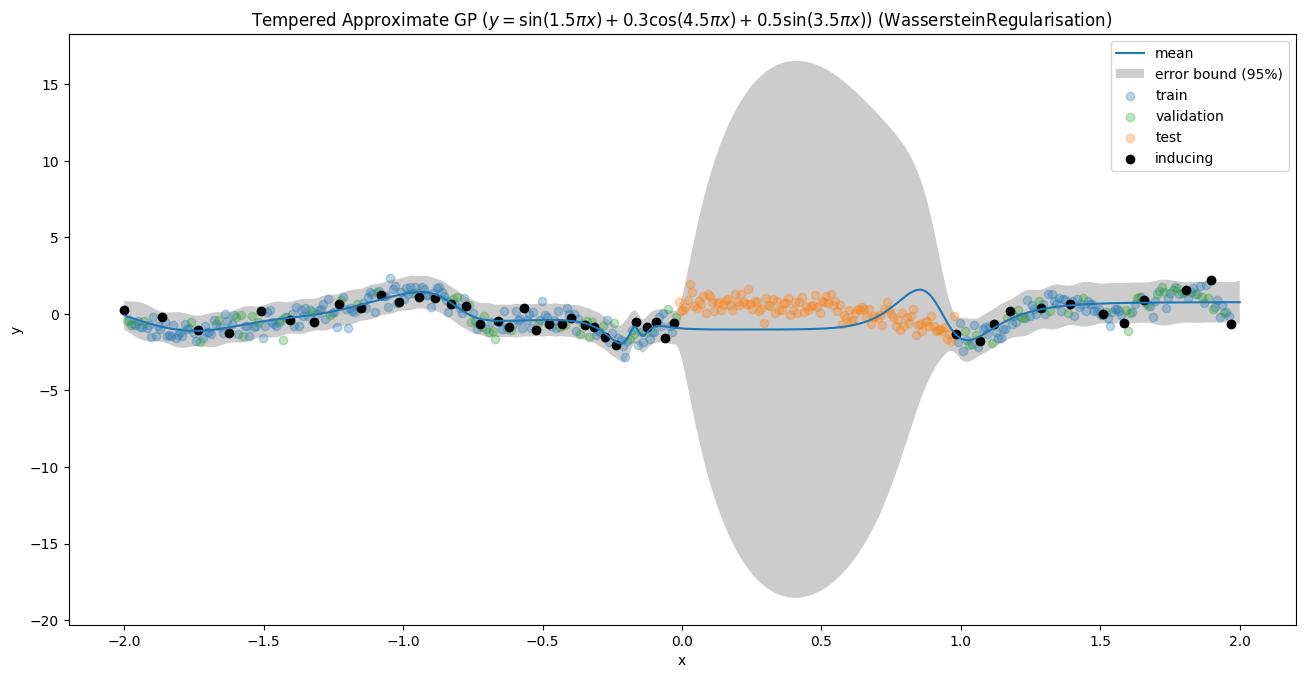
\includegraphics[width=0.9\linewidth]{experiments/regression/toy_curves/outputs/curve3/tempered-WassersteinRegularisation.png}
\end{minipage}%
\begin{minipage}{.5\textwidth}
  \centering
  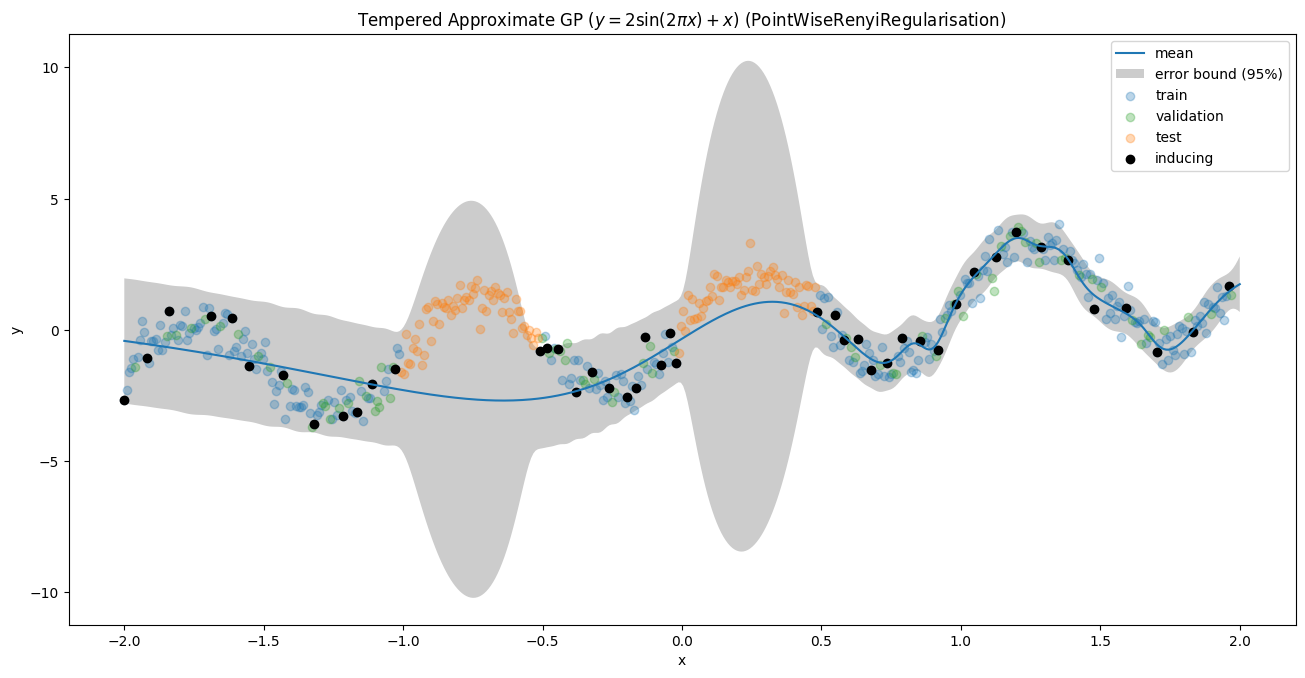
\includegraphics[width=0.9\linewidth]{experiments/regression/toy_curves/outputs/curve4/tempered-PointWiseRenyiRegularisation.png}
\end{minipage}
\caption{Example GVI-GPs for Regression}
\end{figure}
\subsection{Regression Results}

\subsection{Image Classification Results}

\newpage
\section{Future Work}
\subsection{NLP Named-Entity Recognition}
\jw{Putting pre-trained transformers in the mean and kernels.} 


\subsection{Inducing Points Selection}
\subsubsection{Not using actual data points}
\jw{Not selecting actual training points, but learning points that are most representative of the data? i.e. naively a convex combination of images, or weight params in a single layer NN.}
\subsubsection{Selecting in a Feature Space}
\jw{i.e. choosing inducing points from the feature representation of the data points from a NN feature extractor}


\newpage
\section{Conclusions}

\newpage
\bibliography{references}


\newpage
\appendix
\section{Appendix}
\subsection{Positive Semi-Definite Kernels} \label{appendix:positive-definite-kernel}
For a kernel function $k: \mathcal{X} \times \mathcal{X} \rightarrow \mathbb{R}$ defined as an inner product of features in some feature space $\mathcal{H}$:
\begin{align}
    k(x, x') = \langle \phi(x), \phi(x') \rangle_{\mathcal{H}}
\end{align}
where $\phi: \mathcal{X} \rightarrow \mathcal{H}$, a gram matrix $\mathbf{K} \in \mathbb{R}^{N\times N}$ defined element-wise:
\begin{align}
    \left[\mathbf{K}\right]_{n, n'} = k(x_n, x_{n'})
\end{align}
for any $N$ points $\mathbf{X} = \left\{x_n\right\}_{n=1}^N$ with $x_n \in \mathcal{X}$, and any vector $\mathbf{v} \in \mathbb{R}^N$ then:
\begin{align}
    \mathbf{v}^T \mathbf{K} \mathbf{v} &= \sum_{n=1}^N\sum_{n'=1}^N v_n v_{n'}  \left\langle \phi(x_n), \phi(x_{n'}) \right\rangle_{\mathcal{H}} \\
    &= \left\langle\sum_{n=1}^N v_n \phi(x_n), \sum_{n'=1}^N  v_{n'}\phi(x_{n'}) \right\rangle_{\mathcal{H}} \\
    &= \left\| \sum_{n=1}^N v_n \phi(x_n) \right\|^2 \geq 0
\end{align}
showing that $\mathbf{K}$ is a positive semi-definite matrix.

\end{document}